\documentclass[dvipsnames]{article}
\usepackage[english]{babel}
\usepackage{flowchart}
\usepackage{markdown}
\usepackage{soulutf8}
%\usepackage{tabularx}
%\renewcommand{\st}[1]{}
%\usepackage[scale=.75]{geometry}
\usepackage{placeins}
\usepackage{amsthm,amssymb,marginnote}
\usepackage{hyperref}
\hypersetup{breaklinks=true}

\newtheorem{ex}{Example}[section]

\usepackage{subfig}


\usepackage{xcolor}
\newcommand{\nb}[1]{%
  \todo[color=blue!60!black,shadow]{NB:\\ #1}%
}

\usepackage{newunicodechar}

% misc
\newunicodechar{∆}{\ensuremath{\Delta}}
\newunicodechar{⦄}{\ensuremath{\}}}
\newunicodechar{⦃}{\ensuremath{\{}}
\newunicodechar{¯}{\ensuremath{{}^{-}}}
\newunicodechar{·}{\ensuremath{\cdot}}
\newunicodechar{·}{\ensuremath{\cdot}}
\newunicodechar{∫}{\ensuremath{\int}}
\newunicodechar{□}{\Box}
\newunicodechar{⊗}{\ensuremath{\otimes}}
\newunicodechar{★}{\ensuremath{\star}}
\newunicodechar{∗}{^*}
\newunicodechar{♯}{\sharp}
\newunicodechar{①}{(1)}
\newunicodechar{②}{(2)}
\newunicodechar{☺}{\ensuremath{\smiley}}
\newunicodechar{⊣}{\ensuremath{\dashv}}

% advanced typography stuff
\newunicodechar{“}{``}
\newunicodechar{”}{''}
% \newunicodechar{„}{\glqq}


\newunicodechar{fi}{fi}
\newunicodechar{ff}{ff}
\newunicodechar{fl}{fl}
% \newunicodechar{ü}{{\"{u}}}
% \newunicodechar{ä}{{\"{a}}}
% \newunicodechar{ö}{{\"{o}}}
\newunicodechar{∖}{\ensuremath{\setminus}}

%math symbols
\newunicodechar{∃}{\exists}
\newunicodechar{∀}{\ensuremath{\forall}}
\newunicodechar{⇒}{\ensuremath{\Rightarrow}}
\newunicodechar{⇔}{\Leftrightarrow}

% white spaces, etc
%\DeclareUnicodeCharacter{00A0}{~}%\newunicodechar{ }{~}
\newunicodechar{␣}{\_}
\newunicodechar{…}{\ifmmode\dotsc\else\ldots\fi}
\newunicodechar{⋯}{\dotsm}
\newunicodechar{–}{\textendash}


% SUBSCRIPTS
%% letters
\newunicodechar{ₙ}{_n}
\newunicodechar{ₘ}{_m}
\newunicodechar{ₕ}{_h}
\newunicodechar{ᵢ}{_i}
\newunicodechar{ⱼ}{_j}
\newunicodechar{ₖ}{_k}
\newunicodechar{ₜ}{_t}
\newunicodechar{ₛ}{_s}
\newunicodechar{ᵤ}{_u}
\newunicodechar{ᵥ}{_v}
%% numbers
\newunicodechar{₀}{\ensuremath{{}_0}}
\newunicodechar{₁}{\ensuremath{{}_1}}
\newunicodechar{₂}{_2}
\newunicodechar{₆}{_6}

% superscripts
\newunicodechar{ⁿ}{^n}
\newunicodechar{ᵐ}{^m}
\newunicodechar{ˢ}{^s}
\newunicodechar{ᵗ}{\ensuremath{{}^t}}
\newunicodechar{ⁱ}{^i}
\newunicodechar{ʲ}{^j}
\newunicodechar{ᵏ}{^k}
\newunicodechar{ᵗ}{^t}
\newunicodechar{¹}{\ensuremath{{}^1}}
\newunicodechar{²}{^2}
\newunicodechar{³}{^3}
\newunicodechar{ᵀ}{^{\rm T}}


% constants and scalarlike
\newunicodechar{∞}{\infty}

% math operators
%\DeclareUnicodeCharacter{00D7}{\ensuremath{\times}}%\newunicodechar{×}{\times}
\newunicodechar{÷}{\div}
%\DeclareUnicodeCharacter{2190}{\ensuremath\leftarrow}%\newunicodechar{←}{\ensuremath\leftarrow}
%\DeclareUnicodeCharacter{2192}{\ensuremath\rightarrow}%\newunicodechar{→}{\ensuremath\rightarrow}
%\DeclareUnicodeCharacter{21E2}{\ensuremath\dashrightarrow}%\newunicodechar{⇢}{\ensuremath\dashrightarrow}
%\DeclareUnicodeCharacter{21A6}{\ensuremath\mapsto}%\newunicodechar{↦}{\ensuremath\mapsto}
%\DeclareUnicodeCharacter{2196}{\ensuremath\nwarrow}%↖
%\DeclareUnicodeCharacter{2197}{\ensuremath\nearrow}%↗
%\DeclareUnicodeCharacter{2198}{\ensuremath\searrow}%↘
%\DeclareUnicodeCharacter{2199}{\ensuremath\swarrow}%↙
        
% sets 
\newunicodechar{∅}{\varnothing}

% analysis
\newunicodechar{∫}{\int}
\newunicodechar{ℓ}{\ell}

% math relation symbols
\newunicodechar{∈}{\ensuremath{\in}}
\newunicodechar{∉}{\notin}
\newunicodechar{∋}{\ni}
\newunicodechar{≅}{\cong}
\newunicodechar{≥}{\geq}
\newunicodechar{≤}{\leq}
\newunicodechar{≪}{\ll}
\newunicodechar{≫}{\rr}
\newunicodechar{⋘}{\lll}
\newunicodechar{⋙}{\rrr}
%\DeclareUnicodeCharacter{2260}{\neq}%\newunicodechar{≠}{\neq}
\newunicodechar{⊂}{\subset}
\newunicodechar{⊆}{\ensuremath{\subseteq}}
\newunicodechar{⊃}{\supset}
\newunicodechar{⊇}{\supseteq}
\newunicodechar{⊑}{\sqsubseteq}
\newunicodechar{⊒}{\sqsupseteq}

% binary operators
\newunicodechar{⋃}{\bigcup}
\newunicodechar{∪}{\ensuremath{\cup}}
\newunicodechar{⋂}{\bigcap}
\newunicodechar{∩}{\cap}
\newunicodechar{∘}{\circ}

% math arrows 
\newunicodechar{↑}{\ensuremath{\uparrow}}
\newunicodechar{↓}{\ensuremath{\downarrow}}

\newunicodechar{⇀}{\ensuremath{\rightharpoonup}}
\newunicodechar{✉}{\ensuremath{\Letter}}

% summation/products etc (operator for families)
%\DeclareUnicodeCharacter{2211}{\sum}%\newunicodechar{∑}{\sum}
%\DeclareUnicodeCharacter{220F}{\prod}%\newunicodechar{∏}{\prod}

% greek lower case letters (math)
\newunicodechar{α}{\ensuremath{\alpha}}
\newunicodechar{β}{\ensuremath{\beta}}
\newunicodechar{γ}{\ensuremath{\gamma}}
\newunicodechar{δ}{\ensuremath{\delta}}
\newunicodechar{ε}{\ensuremath{\varepsilon}}
\newunicodechar{ϵ}{\ensuremath{\epsilon}}
%\newunicodechar{ϵ}{\varepsilon}
\newunicodechar{η}{\ensuremath{\eta}}
\newunicodechar{λ}{\ensuremath{\lambda}}
\newunicodechar{κ}{\ensuremath{\kappa}}
\newunicodechar{μ}{\ensuremath{\mu}}
\newunicodechar{µ}{\ensuremath{\mu}}
\newunicodechar{ν}{\ensuremath{\nu}}
\newunicodechar{ρ}{\ensuremath{\rho}}
\newunicodechar{σ}{\ensuremath{\sigma}}
\newunicodechar{ξ}{\ensuremath{\xi}}
\newunicodechar{π}{\ensuremath{\pi}}
\newunicodechar{ω}{\ensuremath\omega}
\newunicodechar{ϖ}{\ensuremath{\varpi}}
\newunicodechar{θ}{\ensuremath{\theta}}
\newunicodechar{φ}{\ensuremath{\phi}}
\newunicodechar{ψ}{\ensuremath{\psi}}


% greek upper case letters (math)
\newunicodechar{Θ}{\Theta}
\newunicodechar{Φ}{\ensuremath{\Phi}}
\newunicodechar{Ω}{\Omega}
\newunicodechar{Δ}{\Delta}
\newunicodechar{Σ}{\ensuremath{\Sigma}}
\newunicodechar{Γ}{\ensuremath{\Gamma}}


% calligraphic upper case
\newunicodechar{𝓐}{\ensuremath{\mathcal{A}}}
\newunicodechar{𝓑}{\ensuremath{\mathcal{B}}}
\newunicodechar{𝓒}{\ensuremath{\mathcal{C}}}
\newunicodechar{𝓓}{\ensuremath{\mathcal{D}}}
\newunicodechar{𝓔}{\ensuremath{\mathcal{E}}}
\newunicodechar{𝓕}{\ensuremath{\mathcal{F}}}
\newunicodechar{𝓚}{\ensuremath{\mathcal{K}}}
\newunicodechar{𝓛}{\ensuremath{\mathcal{L}}}
\newunicodechar{𝓝}{\ensuremath{\mathcal{N}}}
\newunicodechar{𝓡}{\ensuremath{\mathcal{R}}}
\newunicodechar{𝓢}{\ensuremath{\mathcal{S}}}
\newunicodechar{𝓧}{\ensuremath{\mathcal{X}}}
\newunicodechar{𝓨}{\ensuremath{\mathcal{Y}}}
\newunicodechar{𝓩}{\ensuremath{\mathcal{Z}}}
\newunicodechar{𝓥}{\ensuremath{\mathcal{V}}}

% fraktur
\newunicodechar{𝕼}{\mathfrak{Q}}

% "normal" boldface
\newunicodechar{𝕍}{\ensuremath{\mathbb{V}}}
\newunicodechar{ℂ}{\ensuremath{\mathbb{C}}}
\newunicodechar{𝔻}{\ensuremath{\mathbb{D}}}
\newunicodechar{𝔼}{\ensuremath{\mathbb{E}}}
\newunicodechar{𝔽}{\ensuremath{\mathbb{F}}}
\newunicodechar{𝕂}{\ensuremath{\mathbb{K}}}
\newunicodechar{ℙ}{\ensuremath{\mathbb{P}}}
\newunicodechar{ℚ}{\ensuremath{\mathbb{Q}}}
\newunicodechar{ℕ}{\ensuremath{\mathbb{N}}}
\newunicodechar{𝕄}{\ensuremath{\mathbb{M}}}
\newunicodechar{ℝ}{\ensuremath{\mathbb{R}}}
\newunicodechar{𝕊}{\ensuremath{\mathbb{S}}}
\newunicodechar{𝕋}{\ensuremath{\mathbb{T}}}
\newunicodechar{ℤ}{\ensuremath{\mathbb{Z}}}
\newunicodechar{𝟙}{\ensuremath{\mathbb{1}}}
\newunicodechar{⨾}{\fatsemi}

\newunicodechar{⟨}{\ensuremath{\langle}}
\newunicodechar{⟩}{\ensuremath{\rangle}}
\newunicodechar{⟪}{\ensuremath{\langle\!\langle}}
\newunicodechar{⟫}{\ensuremath{\rangle\!\rangle}}
\newunicodechar{⌈}{\ensuremath{\lceil}}
\newunicodechar{⌉}{\ensuremath{\rceil}}
\newunicodechar{⌊}{\ensuremath{\lfloor}}
\newunicodechar{⌋}{\ensuremath{\rfloor}}


\newunicodechar{½}{\ensuremath{\sfrac{1}{2}}}
\newunicodechar{ʏ}{\textsc{y}}
\newunicodechar{ᴘ}{\textsc{p}}
\newunicodechar{ʜ}{\textsc{h}}
\newunicodechar{ᴏ}{\textsc{o}}
\newunicodechar{ɴ}{\textsc{n}}

\newunicodechar{‽}{\textinterrobang}
\newunicodechar{⁈}{\textinterrobang}
\newunicodechar{‼}{{\bf \color{red}{!!}}}


%%% Local Variables:
%%% mode: latex
%%% TeX-engine: luatex
%%% TeX-command-extra-options: "-shell-escape"
%%% TeX-master: "HeterogeneousNarwhal"
%%% End:


\usepackage{microtype}
\theoremstyle{definition}
\newtheorem{definition}{Definition}
\usepackage{amsmath}

%\usepackage[utf8]{inputenc}
\usepackage{xspace}
% macros
\newcommand{\xnote}[1]{
  \marginnote{\footnotesize #1}%
}
\newcommand{\rtnote}[1]{%
  \reversemarginpar%
  \xnote{#1}%
  \normalmarginpar%
}

\newcommand{\base}[1][ ]{%
  base ledger%
  \ifthenelse{\equal{#1}{ }}{}{#1}
}
\newcommand{\Base}[1][ ]{%
  Base ledger
  \ifthenelse{\equal{#1}{ }}{}{#1}
}

% \dag is defined to produce † unfortunately
\newcommand{\DAG}[1][]{\textsc{Dag}#1\xspace}
\newcommand{\Dag}[1][]{\textsc{dag}#1\xspace}
\newcommand{\statetright}{\textsf{stateright}}
\newcommand{\Statetright}{\textsf{Stateright}}
\newcommand{\tla}[1][]{\textsc{tla}\ensuremath{{}^{+}}\xspace}

\newcommand{\hnr}{\textsc{hnr}\xspace}
\newcommand{\Hnr}{\textsc{Hnr}\xspace}
\newcommand{\ptop}{\textsc{p\oldstylenums{2}p}}
\newcommand{\Ptop}{\textsc{P\oldstylenums{2}p}}
\newcommand{\fifo}{\textsc{fifo}}

\newcommand{\Fifo}{\textsc{Fifo}}
\newcommand{\aka}[1][]{a.k.a.\xspace}
\newcommand{\ie}[1][, ]{\emph{i.e.}#1}
\newcommand{\eg}[1][, ]{\emph{e.g.}#1}
\newcommand{\Eg}[1][, ]{\emph{E.g.}#1}
\newcommand{\etc}[1][ ]{\emph{etc.}\xspace}
\newcommand{\fig}[1][]{Fig.~}
\newcommand{\Learners}{%
  % the set of learners
  \ensuremath{L}
}
\newcommand{\Q}[1]{%
  % trust live
  Q_{#1}%
}
\newcommand{\rough}[1][ ]{%
  %\fbox{\color{blue!70!black}!!}%
  \ifthenelse{\equal{#1}{ }}%
  {{\color{red}{\bf!!}}}%
  {{\color{blue!70!black}\ul{#1}}}%
}
\newcommand{\circledX}[1]{\tikz[baseline={(x.south)}]{\node[circle,draw,inner sep=.3pt,outer sep=0pt,very thin](x){\tiny #1};}}
\usepackage{newunicodechar}
%\newunicodechar{}{\ensuremath{}}
\newunicodechar{₁}{\ensuremath{{}_1}}
\newunicodechar{₂}{\ensuremath{{}_2}}
\newunicodechar{₃}{\ensuremath{{}_3}}
\newunicodechar{₄}{\ensuremath{{}_4}}
\newunicodechar{₅}{\ensuremath{{}_5}}
\newunicodechar{★}{\ensuremath{*}~}
\newunicodechar{ }{~}
%\newunicodechar{①}{\circledX 1}
\newunicodechar{“}{``}
\newunicodechar{”}{''}
%\newunicodechar{②}{\circledX 2}
\usepackage{stmaryrd}
\newunicodechar{↯}{\lightning}
\newunicodechar{ₐ}{\ifmmode_a\else\ensuremath{{}_a}\fi}
\newunicodechar{ₚ}{\ifmmode_p\else\ensuremath{{}_p}\fi}
\newunicodechar{‼}{\rough}
\newunicodechar{‽}{\ensuremath{?!}}
\newunicodechar{↑}{\ensuremath{\uparrow}}
\newunicodechar{⇑}{\ensuremath{\Uparrow}}
\newunicodechar{♯}{\ensuremath{\sharp%\hat\#
}}
\newunicodechar{∅}{\ensuremath{\varnothing}}
\newunicodechar{≠}{\ensuremath{\neq}}
\newunicodechar{∩}{\ensuremath{\cap}}
\newunicodechar{≡}{\ensuremath{\equiv}}
\newunicodechar{∈}{\ensuremath{\in}}
\newunicodechar{ℝ}{\ensuremath{\mathbb{R}}}
\newunicodechar{↔}{\ensuremath{\leftrightarrows}}
\newunicodechar{→}{\ensuremath{\rightarrow}}
\newunicodechar{⇝}{\ensuremath{\leadsto}}
\newunicodechar{←}{\ensuremath{\leftarrow}}
\newunicodechar{⇒}{\ensuremath{\Rightarrow}}
\newunicodechar{∀}{\ensuremath{\forall}}
\newunicodechar{‌}{\allowbreak }
\newunicodechar{‍}{{}}% non-breaking zero-width space

\usepackage{tikzpeople}%‼ for evil validators etc.

\usepackage{tikz}
\usetikzlibrary{arrows}
\usetikzlibrary{shapes,positioning,fit,backgrounds}
\usetikzlibrary{patterns,intersections,calc}
\newcommand{\qs}[1][~]{\tikz[baseline={([yshift=0pt]theNode.base)}]{\node[rectangle,
,double,inner sep=.5pt,outer sep=0pt,fill=black] (theNode){\textcolor{white}{\footnotesize \bf q#1}};}
}
\newcommand{\bk}[1][green!60!black]{\tikz[baseline={([yshift=0pt]theNode.base)}]{\node[regular polygon, regular polygon sides=6
,double,inner sep=.5pt,outer sep=0pt,fill=#1] (theNode){\textcolor{white}{\footnotesize \bf bk}};}}
\newcommand{\ac}{\tikz[baseline={([yshift=0pt]theNode.base)}]{\node[regular polygon, regular polygon sides=6
,double,inner sep=.5pt,outer sep=0pt,fill=black] (theNode){\textcolor{white}{\footnotesize \bf a}};}}

\newcommand{\hd}[1][ ]{%
  \ifthenelse{\equal{#1}{}}%
  {\tikz[baseline={([yshift=0pt]theNode.base)}]{
      \node[rectangle,inner sep=1.5pt,outer sep=0pt,double] (theNode){\textcolor{black}{\footnotesize \bf \ul{HD}}};
    }}%
  {\tikz[baseline={([yshift=0pt]theNode.base)}]{
      \node[rectangle,double,inner sep=1.5pt,outer sep=0pt,double,draw] (theNode){\textcolor{black}{\footnotesize \bf HD}};
     
    }}%
}
\newcommand{\wh}[1][ ]{%
  \tikz[baseline={([yshift=0pt]theNode.base)}]{%
    \ifthenelse{\equal{#1}{ }}%
    {\node[rectangle,fill=black,inner sep=1.5pt,outer sep=0pt] (theNode){\textcolor{white}{\footnotesize \bf WH}};}%
    {\node[rectangle,rounded corners=0pt,draw,fill=lightgray,inner sep=1.5pt,outer sep=0pt] (theNode){\textcolor{black}{\footnotesize  WH}};}%
  }%
}
\newcommand{\whs}[1][ ]{%
  \ensuremath{\text{\wh[#1]s}}%
}

\newcommand{\anItemInline}[6][theNode]{%
  % #1 the name of the node (just in case, remember picture is on)
  % #2 shape (e.g., ellipse)
  % #3 fill color (e.g., black)
  % #4 draw color (e.g., green, or none)
  % #5 text color (e.g., white)
  % #6 the actual text (e.g., \bf TX)
  \tikz[baseline={([yshift=0pt]#1.base)},remember picture]{%
    \node[fill=#3,draw=#4,inner sep=.5pt,outer sep=0pt,#2] %
    (#1){%
      \textcolor{#5}{%
        \small #6%
      }%
    };%
  }%
  % additional “decorations” via another pic,
  % (with `remember picture` and `overlay`)
  \xspace%
}

\newcommand{\onetx}[1][oneTX]{%
  \anItemInline[#1]%
  {rectangle}%
  {white}%
  {none}%
  {black}%
  {\ul{tx}}%
}

\newcommand{\tx}[1][theTX]{%
  \anItemInline[#1]%
  {rectangle,rounded corners=2pt,inner sep=1pt}%
  {gray}%
  {none}%
  {white}%
  {\textsc{tx}}%
}
\newcommand{\txs}[1][theTX]{%
  \tx[#1]{}\ensuremath{\mathrm{s}}\xspace%
}
\newcommand{\TXS}[1][theTX]{%
  \ensuremath{\overrightarrow{\tx[#1]}}%
}

% \newcommand{\tx}[1][]{%
%   \tikz[baseline={([yshift=0pt]theNode.base)}]{%
%     \node[ellipse,fill=black,inner sep=.5pt,outer sep=0pt] %
%     (theNode){%
%       \textcolor{white}{\footnotesize \bf TX\makebox[0pt][l]{\ensuremath{{}_{#1}}}}};%
%   }%
% }

% \newcommand{\es}{%
%   \tikz[baseline={([yshift=0pt]theNode.base)}]{\node[ellipse,fill=white,draw,thick,inner
%     sep=.5pt,outer sep=0pt] (theNode){\textcolor{black}{\textsc{tx}}};}
% }
\newcommand{\es}[1][theES]{%
  \anItemInline[#1]%
  {rectangle,rounded corners=2pt,inner sep=1pt}%
  {white}%
  {black}%
  {black}%
  {\textsc{tx}}%
}
\newcommand{\rnd}{\ensuremath{\mathrm{rnd}}}
\newcommand{\bn}{\ensuremath{\mathrm{bn}}}
\newcommand{\cnt}{\ensuremath{\mathrm{cnt}}}
% \usepackage{ebgaramond}
% \usepackage[cmintegrals,cmbraces]{newtxmath}
% \usepackage{ebgaramond-maths}
% \usepackage{amssymb}
\usepackage{fontspec}
\setmainfont[SmallCapsFont={Latin Modern Roman Caps}]{Latin Modern Roman}
\addfontfeatures{Numbers=OldStyle}
%\usepackage{unicode-math} // buggy ⁈
%\setmathfont[math-style=ISO,bold-style=ISO,vargreek-shape=TeX]{Latin Modern Math}

%https://tex.stackexchange.com/questions/425098/which-opentype-math-fonts-are-available
\usepackage{comment}
%\includecomment{comment}

\title{%
  Heterogenizing \Dag-based consensus (1/\(n\)):
  \\
  heterogeneous narwhal-rider
}
\author{Typhon Team Heliax}
\date{\today}

\newcommand{\code}[2][ ]{%
  \makebox[0pt][r]{\tiny%
    \href{%
      https://github.com/anoma/typhon/tree/hnarwhal-stateright/hn-stateright/heterogeneous_narwhal%
    }%
    {\color{gray}\texttt{#2}}%
    ~~%
  }%
}
%\renewcommand{\todo}[2][]{}
%\renewcommand{\endnote}[1]{#1}
\usepackage{enotez}
\setenotez{counter-format=Alph,backref=true}

\let\oldendnote\endnote
\renewcommand{\endnote}[2][ ]{%
  \ifthenelse{\equal{#1}{ }}%
  {\marginnote{\oldendnote{#2}}}%
  {\marginnote{\oldendnote[#1]{#2}}}%
}
\newcommand{\hn}{Heterogeneous Narwhal\xspace}
\usepackage[textsize=footnotesize]{./luatodonotes}%\usepackage{todonotes}%


\begin{document}


% \begin{comment}


\begin{center}
  \huge %
  notes to prospective co-authors, %
  colleagues, and friends %
\end{center}
\label{page:firstpage}

\todo[inline, caption={}, color=blue!30!white]{%
  Please note the following about this paper:
  \begin{itemize}
  \item it is “merely” a technical report about
    \emph{Heterogeneous Narwhal}
  \item a “reader's digest” version should follow
  \item it is the \emph{basis} for chimera chains;
  \item however chimera chains, will be left as (concurrent) future work;
  \end{itemize}
  Please keep this in mind,
  when reading the paper!
}

\todo[inline,caption={},color=yellow!50!white]{%
  high-level plan:\\
  \begin{itemize}
    \item  give an operational spec in the main part\\
    \item  state the main properties\\
    \item  defer more technical parts to the appendix and the source code,
    depending on whether it is really a rust-specific implementation detail
    (or it is of conceptual nature)
  \end{itemize}%
}%
\par
\todo[inline,caption={},color=green!30!white]{%
  paper plan (list of ingredients):\\
  \begin{itemize}
  \item “review” learner graph
  \item “review” basic narwhal
  \item
    go for the real deal: %
    we go for an “ideal” world
    where in principle
    every validator
    \begin{enumerate}
    \item could have (part of) all transaction data available
    \item participate in as many differently colored ledgers as desired
    \end{enumerate}
    this goal is independent of the specific uses of the different chains,
    cf. chimera chains
  \item %
    description of the %
    \href{https://github.com/anoma/typhon/tree/hnarwhal-stateright}%
    {prototype implementation}
  \end{itemize}
  \begin{description}
  \item[learner graph] %
    There are several ways to understand the learner graph:
    \begin{itemize}
    \item
      \emph{learner-crafted} learner graphs,
      where learners are formalizing their assumptions about
      \begin{enumerate}
      \item tolerated bad behavior
      \item expected good behavior
      \end{enumerate}
      alternatively,
      for the sake of simplicity,
      one might want to imagine an omniscient observer:
      it ``magically'' give the ``true'' learner-craftable graph to the consensus designer;
      however,
      the more honest version is that
      a learner is in general either
      \begin{itemize}
      \item actively communicate their assumptions (truthfully or not)
      \item ``buy into'' a learner graph, produces by the consensus designer.
      \end{itemize}
      In fact,
      the simplest assumption is the last one:
      the consensus designer also produces the learning graph, %
      which roughly amounts to generating several learner types, %
      such that happy customers will find their match. %
      \\~\\
      \endnote{%
        \texttt{`issue \# 42'} \\
        do we have a principle of corroboration of assumptions?
        \texttt{`issue \# 1,337'} \\
        is there recourse if assumption-contracts are breached? 
      }
    \item
      \emph{observed} learner graphs, %
      typically generated by validators %
      that keep track of what messages have been received,
      are maximally optimistic learner graphs, based on the current (local) observations:
      every validator is supposed to behave well
      unless evidence of misbehaviour/attacks have been found.
      For each (logged/blamable) incident,
      one might actually ask for “compensation action”,
      either investigating an attack,
      admitted misbehavior (typically due to bugs),\endnote{%
        list of types of mistakes that are observable (by validators),
        including resolution/punishing strategies
      }
    \end{itemize}
  \end{description}%
}
\clearpage\cleardoublepage

\maketitle

\begin{abstract}
  \noindent
  Blockchains exhibit \emph{linear} structure
  as each block has a unique reference to \emph{the} previous block.
  If instead,
  each block may reference \emph{several} previous blocks,
  we can build a \emph{directed acyclic graph} (\Dag) of blocks.\xspace%
  \footnote{%
    Note that this includes block chains as one particular case.
  }
  In fact,
  such “block \Dag[s]” are the basic data structure that
  several recent consensus protocols rely on,
  \eg \Dag-rider, Bullshark, and Narwhal\&Tusk.\footnote{%
    The respective references are,
  }
  These protocols build
  a growing “global” \Dag of transaction data such that%
  ---among other things---%
  ① every validator's local view is a sub-\Dag of an “ideal” global \Dag and %
  ② every block of the “ideal” \Dag is
  \emph{logged}\endnote{%
    Logging is terminology borrowed from César Sanchez:
    he likes to talk about \emph{log-chain}s,
    or more verbose “mempool \emph{log system}”
    cite \href{https://arxiv.org/abs/2206.11845}{%
    Setchain: Improving Blockchain Scalability
    with Byzantine Distributed Sets and Barriers}
  }
  for inclusion into a total order of blocks,   %
  which typically implies (eventual) execution of its transactions.

  % Such “global” \Dag[s] will be the topic of the present paper,
  % referred to as {Mempool \Dag[s]}, or \emph{mem-\slshape\Dag[s]},
  % for short.

  The paper focuses on the general principle of heterogenization
  of \Dag-based mempools
  and presents the general idea by means of a specific example,
  which we dub \emph{Heterogeneous Narhwhal-Rider}, or \hnr for short.
  Very much like Heterogeneous Paxos is a heterogeneous version of Lamport's
  Paxos,
  \hnr is a heterogeneous version of
  the Narwhal mempool, extended with \Dag-rider's weak links.
  % In principle,
  % Heterogeneous Narwhal\&Paxos  an alternative for bridges,
  \todo[caption={}]{%
    In a follow up paper,
    we actually need to explain how heterogeneous Narwhal is \\
    1. an alternative to bridges    \\
    2. which benefits / drawback we have, in general\\
    3. which parts are “implementation detail”.\\
    cf. (on page~\pageref{page:firstpage}):
    \textsc{not} part of this paper ...
  }
  % However,
  % in the present paper,
  % we focus on \emph{eventual finality} of the mem-\Dag[s].
  We conclude with a discussion of how heterogenization is a suitable tool
  for building towards an eco-system,
  very much in the spirit of Vitalik Buterin's \texttt{cross-chain
    world}\todo{put in proper term,
    that iscompatible with the Vitalik\\
    cf. Charlotte's ``let's avoid the one big chain'' 
  }.
\end{abstract}

\tableofcontents

\section{Introduction}
Directed acyclic graphs feature in % 
several recently proposed consensus protocols \cite{}.\todo{→isaac?: 
  which ones should I add here?
} %
So, are we presenting yet another \Dag-based consensus protocol?

Clearly, the answer is no; the research is active,
and somebody might be in the very process of writing a new one.
The present paper is rather explains how to heterogenize one example of
\Dag-based mempools;
we believe that this process applies to the whole family of \Dag-based mempools,
which shall dub \Dag-pools. 
So,
for the sake of specificity,
we use a mix of Narwhal and \Dag-rider as a first guinea pig, %
leading up to the general principle of heterogenization.

Along the way,
we shall find out that heterogenization applies differently to questions of availability and integrity \cite{charlotte}:
\begin{description}
\item[availability] all relevant transaction data is promised to be available
\item[integrity] the protocol is safe, \eg no double spends, equivocation,  \etc. 
\end{description}

\todo[inline]{main contribs:\\[\baselineskip]
  \begin{minipage}{1.0\linewidth}
    - general heterogenization principle ...\\
    - ... by virtue of example: Narwhal-\Dag-rider\\
    - [implementation details] \\
    - discussion: alternative to cross-chain bridges (between very different chains ?)
  \end{minipage}\\[\baselineskip]
}

\section{Context}
\label{sec:context}
\todo[inline,caption={}]{.. a little bit of story telling, providing enough context and
  examples such that the reader can picture instances of the abstract concepts
  to be described %
  \begin{itemize}
  \item integrity vs.\ availability
  \item ``learner-graph'' jazz
  \end{itemize}
  Some quotes from Charlotte\endnote{
    Some quotes from Charlotte in the endnotes
      \begin{quote}
    different observers have their own
    beliefs about who might fail, and how
    \\…\\
    Blockchain applications implemented on Charlotte can
    refer to each other’s blocks
    \\…\\
    new mechanisms for \emph{entanglement} of different block histories
    \\…\\
    least
    ordering principle: only that which must be ordered, should be ordered
    \\…\\
    Authenticated Distributed Data Structure (ADDSs)
    \\…\\
    Charlotte ADDSs form the \emph{blockweb}
    \\…\\
    any \emph{observer} can specify their own threat model: %
    the failures they believe the system should securely tolerate. %
    \\…\\
    As a new abstraction layer, Charlotte specifies rules for formatting blocks, referencing
    blocks, and transmitting blocks across the network, and it also offers a formal model for reasoning
    about data integrity and availability.
    \\…\\
    Users can express their assumptions about server behavior (including possible failures)
    \\…\\
    Charlotte to serve as a […] general ADDS framework
    \\…\\
    Charlotte ADDSs can \emph{intersect}, or share blocks
    \\…\\
    “what is the least ordering we actually need?”
    \\…\\
    Charlotte provides a common framework for data structures from separate
    services to \ul{reference each other}.
    \\…\\
    Charlotte data structures are naturally composable: the \emph{union} of two data structures is itself a
    data structure
    \\…\\
    the \emph{intersection} of two data
    structures comprises the data that is part of both structures. We can think of \ul{cross-shard} transactions
    appended to a sharded blockchain ADDS as data in the intersection of multiple shard ADDSs.
  \end{quote}
  }%
}



We want to work towards a multi-chain world in
which
\begin{itemize}
\item everyone can interact with all chains of the ecosystems, %
  and %
\item there is a unique definitive state of every \base.
\end{itemize}

One good example of learners are \emph{executor nodes} %
\cite{anoma_specs}\todo{%
  check / update link, % 
  \href{https://specs.anoma.net/main/components/typhon/execution.html?highlight=exe\#execution}{execution} %
}, %
which are in charge of updating the state of one or several \base. %


For technical considerations,
the main points (for validators and/or executors) are
\begin{itemize}
\item they can participate in the production of as many \base[s] as they want
\item as long as they keep a record of relevant %
  transaction data or the ensuing state changes. %
\end{itemize}

The latter point roughly corresponds to the availability protocol %
while the former is mainly features in the integrity layer. % 
\todo{discuss the general set up of the execution engine / executor nodes:
  these are the prime examples of learners we ``have to'' care about
}

\section{Preliminaries}
\label{sec:preliminaries}
We start with a short review of the central concepts and definitions 
that we rely on in our description of the \hnr protocol.
Moreover,
we also discuss the preliminaries for \hnr's salient properties. 

\todo[inline,caption={}]{%
  ``copy'' relevant parts of %
  the heterogeneous paxos tech report%
  \\
  this can be split up into
  \begin{itemize}
  \item (liveness) qourums -- in the main part
  \item entanglement (for safety) -- in the appendix
  \end{itemize}
}

\subsection{Quorums: learner-specific, global, and universal}
\label{sec:core-defs}

The \hnr protocol is designed to take into account learner-specific assumptions, %
first and foremost about liveness of sets of validators.\xspace%
\footnote{% 
  The terminology about trust assumptions was introduced %
  already for Heterogeneous Paxos \cite{opodis20HPaxos}. %
} %
We start by fixing a finite set of \emph{learners} \(\Learners\); %
each learner holds certain beliefs %
and these beliefs impose restrictions on %
the behavior of validators that is deemed possible.\xspace%
\todo{%
  double check with Isaac %
  that it is safe to use the terms %
  validator and acceptor %
  interchangeably %
}%
Each learner is asked to commit to a set of \emph{quorums}\xspace%
\todo{define\&explain}%
such that at least one of the quorums will be live at all times. %
\endnote{
  this is way too strong as an assumption, no ?
}
\endnote{%
  on corroboration of liveness assumptions: %
  keep tabs on that there is enough progress
  that 
  \\-- \emph{could} stem from one of the quorums 
  \\-- \emph{has to} stem from one of the quorums 
}%
\endnote{%
  on blamable violations of liveness: %
  it seems impossible to prove that liveness assumptions are wrong, %
  unless we reduce liveness to safety, 
  by adding absolute limits for latency of responses 
  (which on top requires network synchrony)
}
In particular,
the protocol description takes as input a function
from learners to sets of (learner-specific) quorums.
Let us mention once more, %
as protocol designers, % 
we assume each learner to have commited to a set of quorums, %
such that one of these quorums is live at all times %
(and that this is compatible with the learner's believes).\xspace%
\footnote{%
  This is formalized as
  \href%
  {https://github.com/anoma/typhon/blob/main/tla/HPaxos.tla\#L34}%
  {\texttt{Trust Live}}
  in the
  \href%
  {https://github.com/anoma/typhon/blob/main/tla/HPaxos.tla\#L34}%
  {\tla-specification}. 
}




\begin{definition}[Learner-specific quorum system]
  \label{def:trustlive}
  A \emph{learner-specific quorum system} is a function from 
  learners to sets of quorums.
  For a {learner-specific quorum system}~\(\Q{}\)
  and a learner \(a\), 
  we denote the learner's set of qourums by \(\Q{a}\), 
  whose elements are the \emph{learner-specific quorums} of \(a\).
  We use \(qₐ, q'ₐ,\) \etc to range over learner-specific quorums of learner \(a\).
\end{definition} %
One might even go as far and ask learners to choose %
a maximal set of quorums that is compatible with their beliefs; %
however, %
all we need is a map from learners to sets of quorums. %

Now, based on quorums systems, 
we can formulate the remaining two core definitions. %
Global weak quorums are important for matters of availability:
if a global weak quorum is holding a copy of a particular transaction request, %
then one copy should be available %
(as a ``shared belief'' of all learners). %
\begin{definition}[Global weak quorum]
  \label{def:global-weak-quorum}
  A \emph{global weak quorum} is %
  a set of validators \(X\) that is a weak quorum for each learner, %
  i.e., 
  for every learner~\(a ∈ \Learners\) and %
  all learner-specific quorums \(qₐ ∈ \Q{a}\), %
  we have a non-empty intersection \(X ∩ qₐ ≠ ∅\). %
\end{definition}


\todo{explain where we need universal quorums}%
\begin{definition}[Universal Quorum]
  \label{def:universal-quorum}
  A \emph{universal quorum} is a set of quorums
  that contains at least one learner-specific quorum for each learner.
\end{definition}

\subsection{Discussion of desirable properties}
\label{sec:property-discussion}

\todo[inline,caption={}]{%
  recall/discuss the properties 
  such as chain quality, 
  fair inclusion,
  \etc
}


\section{Overview: %
  mem-DAGs, heterogeneity, etc.
}
\label{sec:overview}
\todo[inline,caption={}]{probably move the below ``hidden material'' (see \TeX-source)
  to an earlier point (context)}
\begin{comment}
Recall that we aim to build “global” \Dag[s] of blocks, one for each leaner, 
each referencing a quorum of previous blocks (of the respective learner);
note that he term global is problematic insofar 
as only a fictive omniscient observer
that sees all blocks that some validator may know it.
However,
the global \dag is of intersubjective relevance,
as every \emph{local} view of any validator
is a sub-graph of the “global” \Dag.
Put differently,
all local \Dag[s] are expected to be consistent
in the sense as it makes sense to talk about the union of the (logical) \dag[s]. 

A block in the \Dag can be \emph{committed}
using an arbitrary consensus algorithm
if it is referenced by a weak quorum
(from the next “layer” in the \Dag)
in every local view of the consensus participants.

An example of such a “global” \Dag
is shown in \fig\ref{fig:blue_dag}.
In the present paper,
we describe a protocol for concurrent building
of \emph{entangled} \Dag[s] for a whole ecosystem of different ledgers,
in the spirit of a multi-chain world.

\begin{figure}[htb]
  \centering
  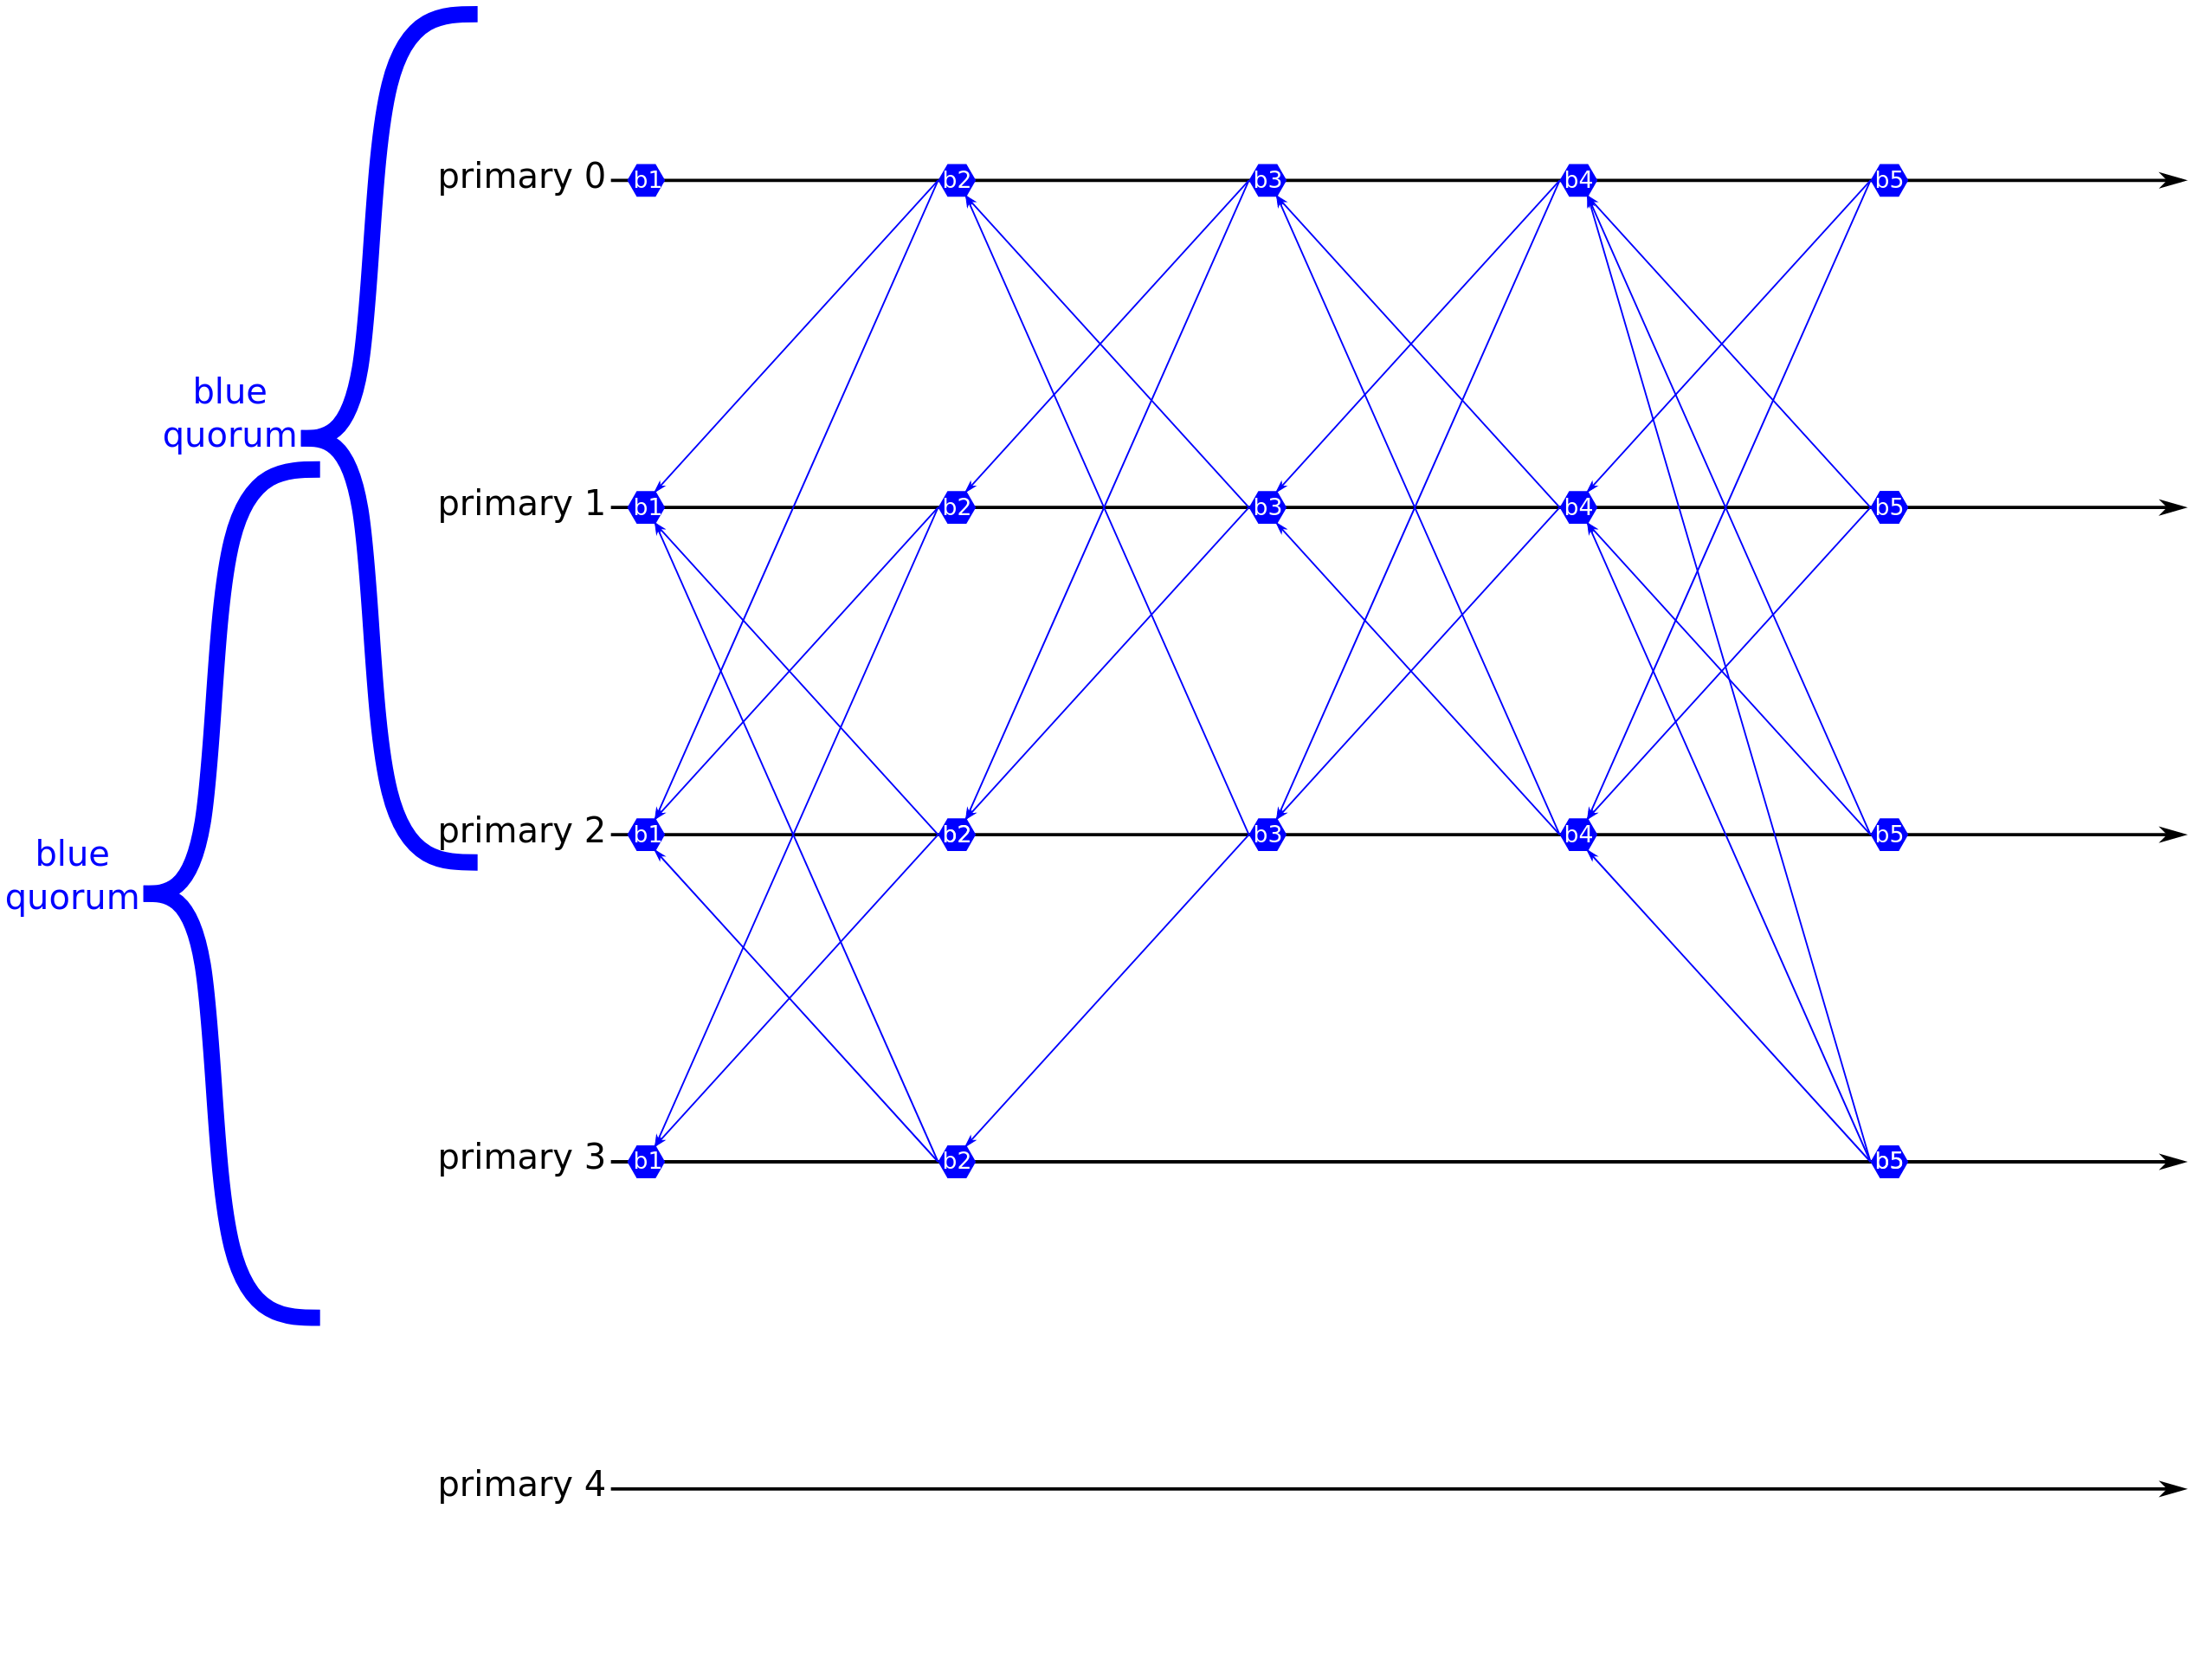
\includegraphics[width=.95\linewidth]{./blue_dag.png}
  \caption{A mem-\Dag (self-references omitted)}
  \label{fig:blue_dag}
\end{figure}


\begin{figure}[htb]
  \centering
  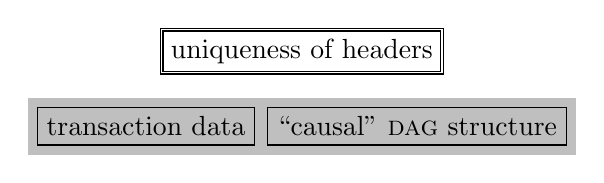
\begin{tikzpicture}
    \node[draw] (avl) {transaction data};

    \node[draw,right=1ex of avl] (dag) {``causal'' \Dag structure};
    \begin{pgfonlayer}{background}
    \node (x) [fill=lightgray,fit=(avl)(dag)] {};
  \end{pgfonlayer}
  \node[above=2ex of x,draw,double] {uniqueness of headers};
\end{tikzpicture}\makebox[0pt][r]{\Large \bf \color{blue} make this Fig. something that actually helps (or delete)} \protect\todo{where to put the signed quorums ?!}
  \caption%
  [Interdependence of availability and integrity]%
  {Illustration of
    the interdependence of the availability and
    integrity protocols}
  \label{fig:availability-n-integrity}
\end{figure}



Roughly, we have two complementary protocols running concurrently:
 \begin{enumerate}
 \item the availability protocol; and
 \item the integrity protocol.
 \end{enumerate}
 The availability protocol makes sure
 that transaction data is available
 as long as necessary;\footnote{%
   There is some fine print concerning
   the conditions under which this is actually the case.
 }
 moreover,
 the availability protocol
 is tasked with keeping available
 the \emph{signed headers},
 \todo{explain \texttt{signed headers}}
 which the integrity protocol produces.

 The integrity protocol makes sure that
 each validator can only produce one block in each of its (local) rounds.


\end{comment}
\section{Architecture and communication patterns}
\label{sec:communication-patterns}
 \Hnr incorporates Narwhal's~\cite{NT}
 scale out architecture: %
 each validator has a unique \emph{primary} and %
 a number of \emph{workers} %
 (see \fig\ref{fig:validators}).
\begin{figure}[htb]
  \centering

validator:\(\left\{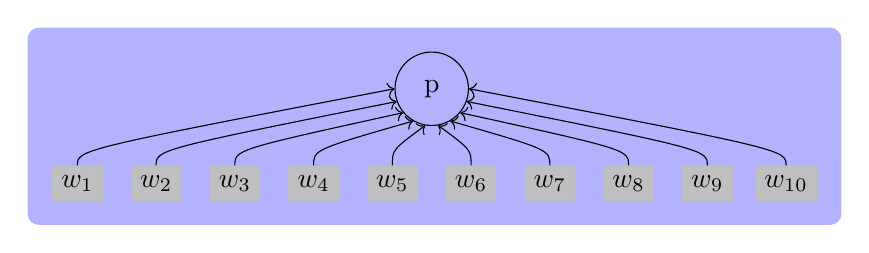
\begin{tikzpicture}[baseline={(p.south)},remember picture]
    \node[circle,draw,inner sep=1.5ex] (p) at (5.5,1.2) {p};
    \foreach \i in {1,...,10}{
      \coordinate (p_\i) at  (p.160+20*\i);
    }
    \foreach \i in {1,...,10}{
      \node[rectangle,fill=lightgray](w_\i) at (\i,0){\(w_{\i}\)};
      \draw[->] (w_\i.north) .. controls +(0,.2) .. (p_\i);
    }
    \begin{pgfonlayer}{background}
      \node[rounded corners,fill=blue!30!white,inner sep=2ex] (background) [fit=(w_1.south west)(w_10.south east)(p)] {};
    \end{pgfonlayer}
  \end{tikzpicture}\right.\)
\vspace{4ex}

\tikz[remember picture]{\node[rectangle,fill=gray,draw] (c) {client};}\hfill~\\

\vspace{4ex}

validator:\(\left\{\begin{tikzpicture}[baseline={(q.north)},remember picture,yscale=-1]
    \node[circle,draw,inner sep=1.5ex] (q) at (5.5,1.2) {q};
    \foreach \i in {1,...,10}{
      \coordinate (q_\i) at  (q.200-20*\i);
    }
    \foreach \i in {1,...,10}{
      \node[rectangle,fill=lightgray](v_\i) at (\i,0){\(v_{\i}\)};
      \draw[->] (v_\i.south) .. controls +(0,.2) .. (q_\i);
    }
    \begin{pgfonlayer}{background}
      \node[rounded corners,fill=blue!30!white,inner sep=2ex] (background) [fit=(v_1.north west)(v_10.north east)(q)] {};
    \end{pgfonlayer}
    % --------------------------------------------------------------------------------
    \begin{scope}[overlay,thick]
          \foreach \j in {1,...,10}
    \draw[<->] (v_\j) -- (w_\j);

    \draw[<->] (c.-15) .. controls +(2,0) and +(-1,-1) .. (v_3.north west);
    \draw[<->] (c.15) .. controls +(2,0) and +(-1,1).. (w_7.south west);
    \draw[<->] (p) -- (q);
    \end{scope}
  \end{tikzpicture}\right.\)
  \caption{The structure and communication patterns of validators}
  \label{fig:validators}
\end{figure}




\section{Worker actions (availability protocol)}
\label{sec:worker-actions}
Every validator has the same number of workers.
Thus,
each worker can be assigned a unique \emph{mirror worker}
on every other validator.
We shall adopt the convention
that mirror worker identifiers share the same subscript.
For example,
in \fig\ref{fig:validators},
workers~\(w_2\) and~\(v_2\) are mirror workers of each other.
Workers are mainly featuring in the availability protocol; %
their role in the integrity protocol concerns ``mere bookkeeping'' only. % 
Specifically,
workers keep track of (batches of) transactions,
their hashes,
and erasure coding shares---which shall be trivial, along the lines
of~\cite{NT}.
The only information that workers provide to their primaries  %
are hash references to transaction request data. %
In this way,
we can save network bandwidth usage of primaries. %
Moreover,
as a secondary principle, %
primaries never send messages or other direct signals to their workers.\xspace%
\footnote{%
  However, %
  workers receive signals upon successful execution of transactions, 
  which allows them to free up the transaction storage. 
}%
\todo{add some short discussion about executor nodes, \etc }
\endnote{%
  Sharing the round number is the point where
  one might be tempted to deviate from the principle that
  validators never talk back to their workers
  (\emph{qua validator} -- the executor nodes on a validator do talk back).
}

\subsection{Pre-execution protocol}
\label{sec:base-protocol}
\todo[inline]{%
  we need to ``announce'' headers
  ---
  in contrast to what what is/was in the specs
  \tiny\tt(written March 7 2023, Tobias Heindel)
}
\todo[inline]{%
  so, signed qourums are an ``output'' of the integrity protocol,
  and need to be made available
  (such that it is possible to create new headers).
  NEEDS EXPLAIN
}

\todo[inline]{%
  worker hashes also should include an availability certificate %
  of the header creator's previous header %
  \\
  However,
  as we now have the header announcement, 
  one could logically move it to the primary's signature request ?
}
\todo[inline,color=green!80!black]{
  defer all the data structure talk to the section on 
  message dependency management
  Section/Appendix\ref{sec:mess-depend-manag}
}
\todo[inline,color=yellow!80!white]{
  \# issue:
  we are still missing information about 
  how long data has to be stored.
  We might also want to defer this too
  Section/Appendix\ref{sec:mess-depend-manag}
}
\begin{description}
\item[%
  \code{MessageEnum::TxReq}%
  Transaction request collection ({\tx}←)%
  ]
  \xnote{worker\\ ← client}
  \todo{in the typhon sources for \texttt{`heterogeneous\_narwhal`},
    each transaction collection is \emph{immediately} followed
    by a \texttt{TxAck}
  }
  Each worker keeps listening
  for incoming transaction requests from clients.\footnote{%
    The bandwith and amount of storage for storing incoming transactions 
    \emph{should} be big enough
    to process all incoming transactions.
    We share this assumption with Byzantine set consensus \cite{RedBelly}.
    Transaction fees are one way to avoid flooding attacks,
    making the latter prohibitively expensive.
    For example,
    we might consider using a \fifo-buffer; %
    however a priority queue that takes into account a combination of %
    fees and quality of service considerations %
    is more suitable for managing the flow of incoming transaction requests.
  }
  Transaction requests should be buffered using reasonably fast memory % 
  (to ensure that all requests are eventually served); %
  transaction request fees may be imposed %
  to control the rate of client requests. %
  \endnote{%
    The matter of reasonably fast transaction buffer
    needs additional context,
    possibly involving more specifics from the \ptop layer.
  }
  \begin{description}
  \item[\code{MessageEnum::TxAck}
    Transaction request acknowledgment]
    Optionally, %
    one may acknowledge the client's requests. 
    \todo[inline,color=SkyBlue]{%
      In the
      \href{https://github.com/anoma/typhon/tree/hnarwhal-stateright/hn-stateright/heterogeneous_narwhal}%
      {code},
      we instantly acknowledge each received transaction
      by sending a message back to the sender of the transaction request.
    }
  \item[%
    \code{???}%
    {Transaction batching (\(\txs:= \txs:\tx\))}%
    ]%
    \xnote{[worker]}%
    Every worker stores the received transaction request to %
    \emph{the} current batch \txs, %
    which is essentially a (possibly empty) list of transaction requests. %
    The worker adds the transaction request \tx to the current batch \txs. %
    This happens unconditionally,
    \ie there is always a unique current transaction batch \
    and every transaction request has to be added to the current batch. %
    New batches may be created over time, %
    but each batch in this ``stream'' of batches has a unique number.
    Within a batch, %
    transactions are assigned consecutive sequence numbers; %
    the sequence number of a transaction is essentially the position in the
    current batch. %
    Thus,
    each transaction request to a fixed worker can by identified by
    its \emph{batch} and \emph{sequence number}. 
  \item[%
    \code{TxToAll}%
    {Transaction broadcasting (\tx{}⇝\es{}⇒)}%
    ]%
    \xnote{%
      worker\\
      ⇒worker
    }%
    Each received transaction request is broadcast to all mirror workers.
    In principle,
    we could use arbitrary erasure coding schemes.
    However,
    in line with the original version of Narwhal \cite{NT}, %
    we use full copies as erasure codes.
    Despite the coincidence of erasure codes and the ``original'' data, %
    we visually distinguish the “copy” of a transaction
    from the “original” transaction supplied by the client, 
    using two different symbols, namely \tx\ and \es, respectively. %
    When broadcasting copies of received transaction requests,
    the message also provides the current batch number and %
    the sequence number of the transaction within this batch. %
  \item[%
    \code{WHxToAll,WorkerHx}%
    {Worker hash broadcast (\tx{!}\wh{}↑⇒)}%
    ]%
    \xnote{worker%
      \\⇒ worker%
      \\→ primary%
    }
    When a worker receives a transaction request,
    this might trigger a new worker hash to be produced %
    (if it is ``time''\xspace%
    \footnote{%
      \label{fn:time}
      At which exact moment worker hashes are compiled can depend on several
      factors, 
      \eg on a maximum number of transaction requests per worker hash 
      or a maximum delay between the first and the last transaction request within a worker hash.
    }
    to do so).
    In principle,
    it is up to the worker to decide,
    as long as each worker hash contains at least one transaction. %
    The worker hash broadcast involves the following steps: %
    \begin{enumerate}
    \item broadcasting the new worker hash to mirror workers; %
    \item sending the new worker hash to the worker's primary; %
    \item resetting the current transaction request buffer to the empty list; %
    \item incrementing the batch number; %
    \item last, but not least, %
      storing the transactions of the current batch for retrieval. %
      \todo{%
        The present state of the specs (in flux),
        we notify workers for matters of executing at the level of single transactions
      }
    \end{enumerate}%
    {}\code{WorkerHashData,WorkerHashSignature}%
    The new worker hash consists of
    \begin{itemize}
    \item the hash of the current batch \txs, %
    \item the length of the current batch, %
    \item the identifier of the current worker, %
    \item a signature of the above data by the current worker. %
    \end{itemize}
  \end{description}
  \endnote{%
    If we want to perform proper erasure coding,
    we also have to replace a full broadcast by
    something more sophisticated.
    \Eg each mirror worker receives a different message.
    We first cover the case of trivial erasure coding
    ‼[covering the case of proper erasure codining in ‽].
  }

\item[%
  \code{MessageEnum::TxToAll}%
  Transaction copy (\es{}←)%
  ]\xnote{%
    worker\\
    ←worker
  }%
  For the proper handling of transaction copies and worker hashes
  of mirror workers,
  we keep for each mirror worker
  a set of \emph{active batch numbers}
  and a map from active batch numbers to
  a set of (ranges of) sequence numbers of received transactions in that batch,
  paired with a worker hash option,
  depending on whether or not we have received the corresponding worker hash. 
  \begin{description}
  \item[Transaction storage] 
    Upon receiving a transaction copy, %
    the worker has to store the copy locally %
    such that it can be retrieved quickly via
    \begin{itemize}
    \item the \textsc{id} of the collecting worker, 
    \item the batch number of the batch to which it belongs, and
    \item the sequence number within the batch to which it belongs.
    \end{itemize}
    Note that copies of transactions are \emph{not} signed by the worker. %
    Signatures are deferred to worker hash broadcast. % 
    Storing transaction copies as above will be useful %
    for handling ``foreign'' worker hashes, %
    \ie worker hashes that refer to transactions that are collected at other
    workers. 

  \item[\code{WHxFwd}{Worker hash forwarding (\es!\wh[]↑)}] 
    \xnote{%
      worker\\
      →primary%
    }
    In case, %
    the transaction was the last missing one to match a previously received worker hash, %
    the worker hash is ``forwarded'' to its primary. %
  \end{description}

% \item[Worker hash compilation (\wh)]
%   \xnote{(worker)}
%   Towards the end of a “validator round”,\endnote{%
%     Is there any such thing as “validator round”?\\
%     - sequence number\\
%     - validator height\\
%     - ...
%   }%
%   \todo[inline,color=red,caption={}]{%
%     here now, we need to
%     \begin{enumerate}
%     \item introduce signals from primary to workers,
%     \item replace the round number by a “take” based mechanism
%     \end{enumerate}
%   }
%   \xspace
%   each worker produces its worker hash for the broadcast batch of transactions.
%   In detail,
%   a worker hash consists of
%   \begin{itemize}
%   \item the hash of the broadcast list of transactions,
%   \item the number of transactions, and
%   \item the \st{round number}\ul{take},
%     \todo[color=SkyBlue]{%
%       very much like in a movie,
%       we piece together each header form \textsc{take},
%       or any other single word for \emph{batch number}
%       }
%   \end{itemize}
%   signed by the worker.
%   \endnote{\color{red}
%     For general erasure coding:
%     \em Does this need to includes for each receiving worker,
%     the (hashes of the) erasure coding shares that
%     they should have available. ?
%   }

\item[%
  \code{WHxToAll}%
  Worker hash ({\wh[]←})%
  ]%
  \xnote{%
    worker\\%
    ← worker%
  }
  When a worker receives a worker hash from a mirror worker, %
  it updates the worker hash storage.

  \begin{description}
  \item[%
    \code{MessageEnum::WHxFwd}%
    Worker hash forwarding ({\wh[]!\wh[]↑})%
    ]
    \xnote{worker\\ → primary} 
    If a worker has already stored the transactions of a received worker hash, %
    it “forwards” the worker hash to its primary.\footnote{%
      Validators will use this information
      to send availability commitments to block headers of other primaries.
    }
  \end{description}
\end{description}

Recall that we have emphasized what workers do in reaction to \emph{receiving}
messages, %
such that sending a message might be the final step of several, slightly
different scenarios %
(depending of which message from a \emph{set} of triggering messages arrives
last and thus becomes \emph{the} trigger). %

\begin{figure}[htb]
  \centering
  \todo[inline,caption={}]{%
    \begin{itemize}
    \item need to ``fix'' the \tx subscripts to be sequence numbers;
      possibly adding also the batch number of the worker hash?
    \item header announcements only need to send ``fingerprints'' of headers,
      for the moment represented by \(\wh[]^*\)
    \end{itemize}
  }
  %
  \tikzstyle{every node}+=[outer sep=0pt,inner sep=1pt]
  \newcommand{\primaryDistance}{15ex}
  \newcommand{\workerPrimaryDistance}{1ex}
  \newcommand{\workerDistance}{3ex}
  \scalebox{.9}{%
  \footnotesize%
  \begin{tikzpicture}[scale=1.2]
    %%%%%%%%%%%%%%%%%%%%%%%%%%%%%%%%%%%%%%%%%%%%%%%%%%%%%%%%%%%%%%%%%%%%%%%%%%%%%%%%
    % The message passing diagram of the availability protocol at genesis
    %%%%%%%%%%%%%%%%%%%%%%%%%%%%%%%%%%%%%%%%%%%%%%%%%%%%%%%%%%%%%%%%%%%%%%%%%%%%%%%%
    % first the time lines for primaries and their workers
    \coordinate (primaryAnchor) at (0,0);
    \foreach \p in {1,...,5} {
      \node[below=\primaryDistance of primaryAnchor,anchor=east] (p\p)
      at (primaryAnchor) {\ensuremath{\text{primary}_\p}};
      \draw[->] (p\p) -- ++(10.4,0);
      \coordinate (workerAnchor) at ([yshift=-\workerPrimaryDistance]p\p.east);
      \foreach \j in {1,...,2} {
        \node[below=\workerDistance of primaryAnchor,anchor=east] (w\p_\j)
        at (workerAnchor) {\ensuremath{\text{worker}_{\p,\j}}};
        \draw[->,draw=lightgray,semithick] (w\p_\j) -- ++(10.4,0) ;
        \coordinate (workerAnchor) at (w\p_\j.east);
      }
      \coordinate (primaryAnchor) at (p\p.east);
    }
    %%%%%%%%%%%%%%%%%%%%%%%%%%%%%%%%%%%%%%%%%%%%%%%%%%%%%%%%%%%%%%%%%%%%%%%%%%%%%%%%
    % a first transaction tx1
    \node (tx1) at ([xshift=3.5ex]w1_1.east) {\tx₁};
    \draw[->,double,dotted,shorten >=-2ex] (tx1.200) ++ (200:1em) -- (tx1);
    \foreach \p in {2,...,5} {
      \node (es\p_1) at ([xshift=6ex-\p ex]tx1|-w\p_1) {\es₁};
      \draw[->] (tx1) -- (es\p_1) ;
    }
    % a bunch of transactions tx2-5 that will make it into WHs actually
    \node (tx2) at ([xshift=3*3.5ex]w3_2.east) {\tx₂};
    \draw[->,double,dotted,shorten >=-2ex] (tx2.200) ++ (200:1em) -- (tx2);
    \foreach \p in {1,2,4,5} {
      \node (es\p_2) at ([xshift=6ex-\p ex]tx2|-w\p_2) {\es₂};
      \draw[->] (tx2) -- (es\p_2) ;
    }
    \node (tx3) at ([xshift=5*3.5ex]w3_2.east) {\tx₃};
    \draw[->,double,dotted,shorten >=-2ex] (tx3.200) ++ (200:1em) -- (tx3);
    \foreach \p in {1,2,4,5} {
      \node (es\p_3) at ([xshift=6ex-\p ex]tx3|-w\p_2) {\es₃};
      \draw[->] (tx3) -- (es\p_3) ;
    }
    \node (tx4) at ([xshift=7*3.5ex]w3_1.east) {\tx₄};
    \draw[->,double,dotted,shorten >=-2ex] (tx4.200) ++ (200:1em) -- (tx4);
    \foreach \p in {1,2,4,5} {
      \node (es\p_4) at ([xshift=6ex-\p ex]tx4|-w\p_1) {\es₄};
      \draw[->] (tx4) -- (es\p_4) ;
    }
    \node (tx5) at ([xshift=9*3.5ex]w3_1.east) {\tx₅};
    \draw[->,double,dotted,shorten >=-2ex] (tx5.200) ++ (200:1em) -- (tx5);
    \foreach \p in {1,2,4,5} {
      \node (es\p_5) at ([xshift=6ex-\p ex]tx5|-w\p_1) {\es₅};
      \draw[->] (tx5) -- (es\p_5) ;
    }
    % collection of txs into worker hashes wh1 and wh2
    \node[right=.1ex of tx5] (wh1) {\wh₁};
    \draw[dotted,bend right=2.5ex] (wh1.center) to (tx5.center);
    \draw[dotted,bend right=5ex] (wh1.center) to (tx4.center);
    \node[right=3.5ex of wh1|-tx3] (wh2) {\wh₂};
    \draw[dotted,bend left=2.5ex] (wh2.center) to (tx3.center);
    \draw[dotted,bend left=5ex] (wh2.center) to (tx2.center);
    %%%%%%%%%%%%%%%%%%%%%%%%%%%%%%%%%%%%%%%%%%%%%%%%%%%%%%%%%%%%%%%%%%%%%%%%%%%%%%%%
    % "upload" of worker hashes wh1 and wh2 to the primary, wh1' and wh2'
    \node (wh1') at ([xshift=-2ex]wh2|-p3) {\wh₁};
    \draw[->] (wh1) -- (wh1');
    \node[right=0ex of wh1'] (wh2') {\wh₂};
    \draw[->] (wh2) -- (wh2');
    % the following should be much later, but ... (unique harmless hack)
    \node[right=1ex of wh2',fill=white] (hd3) {{\hd[]}};
    \foreach \k in {1,2}
    \draw[dotted,bend right=9ex-3*\k ex] (hd3) to (wh\k'.center);
    %%%%%%%%%%%%%%%%%%%%%%%%%%%%%%%%%%%%%%%%%%%%%%%%%%%%%%%%%%%%%%%%%%%%%%%%%%%%%%%%
    % dissemination of worker hashes wh1 and wh2
    \foreach \p in {1,2,4,5} {
      \node (wh1_\p_1) at ([xshift=3ex-\p ex]wh1'|-w\p_1) {\wh[]₁};
      \draw[->] (wh1) -- (wh1_\p_1) ;
    }
    \foreach \p in {1,2,4,5} {
      \node (wh2_\p_2) at ([xshift=6ex-\p ex]wh2'|-w\p_2) {\wh[]₂};
      \draw[->] (wh2) -- (wh2_\p_2) ;
    }
    %%%%%%%%%%%%%%%%%%%%%%%%%%%%%%%%%%%%%%%%%%%%%%%%%%%%%%%%%%%%%%%%%%%%%%%%%%%%%%%%
    % worker hash upload at receiving validators
    \foreach \whx in {1,2} { % for each of the two worker hashes
      \foreach \p in {1,2,4,5} { % for each "other" validator
        \node (wh\whx_\p_\whx') at ([xshift=4ex-\whx ex]wh\whx_\p_\whx|-p\p) {\wh[]\ensuremath{{}_\whx}};
        \draw[->] (wh\whx_\p_\whx) -- (wh\whx_\p_\whx');
        % and header creation (after second block)
        % ... and sending availability votes
        \ifthenelse{\equal{\whx}{2}}%
        {\node[right=2ex of wh\whx_\p_\whx',fill=white,draw=none] (hd\p) {\({\hd[]}^*\)};
          \foreach \k in {1,2}
          \draw[dotted,bend right=9ex-3*\k ex] (hd\p) to (wh\k_\p_\k'.center);
        }%
        {}%
      }
    }
    %%%%%%%%%%%%%%%%%%%%%%%%%%%%%%%%%%%%%%%%%%%%%%%%%%%%%%%%%%%%%%%%%%%%%%%%%%%%%%%%
    % collect "foreign" whs into availability votes for a block
    \coordinate (ac) at ([xshift=2ex,yshift=2ex]hd1|-p3);
    \foreach \p in {1,2,4} { % for each "other" validator
      \node[fill=white] (av\p) at (ac){{\hd[]}\makebox[0pt][l]{\ensuremath{{}_{\sim\p}}}};
      \coordinate (ac) at ([xshift=-1ex,yshift=-1ex]ac);
    }
    \foreach \p in {1,2,4} { % for each "other" validator
      \draw[->] (hd\p) -- (av\p.east);
      \draw[%ultra thick,red,double,
      ->] (hd3) --
      % node[auto]{trigger}
      (hd\p);
    }
    \draw[%ultra thick,red,double,
    ->] (hd3) --%node[auto]{trigger} 
    (hd5);
    \node[fill=white] (av3) at (ac){{\hd[]}\makebox[0pt][l]{\ensuremath{{}_{\sim3}}}};
    \draw[->] (hd3) -- (av3);
    \begin{pgfonlayer}{background}
      \node[fit={(av3)(av1)([xshift=2ex]av1.north east)},fill=lightgray] (ac3) {};
    \end{pgfonlayer}
    % broadcast the availability certificate
    \foreach \p in {1,...,5} { % for each "other" validator
      \node (ac\p') at ([xshift=17ex-\p ex]ac|-p\p) {\ac\ensuremath{{}_\p}};
      \draw[->] ([yshift=2.5ex-\p ex]ac3.east) -- (ac\p');
    }
  \end{tikzpicture}%
  }
  \caption{The availability protocol in the genesis round}
  \label{fig:availability-protocol}
\end{figure}
\todo[caption={}]{%
  concerning ``triggering'' the header construction,
  there are the following points
  \\
  1. when a the triggering signing request is \emph{received} by a primary,
  we might need to ``wait'' for the corresponding worker hashes
  \\
  2. new signing for more recent rounds make old ones obsolete
  \\
  3. what are the incentives for speedy signing ?
}\endnote{%
  On speedy signing incentives:
  \begin{itemize}
  \item as a validator, I want primarily \emph{my} blocks signed
  \item
    So, why should I sign \emph{your} header?!
    \begin{itemize}
    \item It comes even with the storage commitment for my workers!
    \item Actually, if “everybody” else is signing, I am still gonna be fine !!!
    \end{itemize}

    Thus, having a signature as part of an availability certificate should give
    some kind of reward!
  \end{itemize}
  On the other hand,
  it is natural to collect signatures for the availability certificate
  on a “first come, first served” basis
}
%\end{comment}
\subsection{Execution support protocol}
\label{sec:exe-supp-protocol}

\todo{todo!}
\section{Primary actions}
\label{sec:primary-actions}

Primaries will follow a protocol %
in which we can distinguish between matters of availability %
and matters of integrity. %
For the availability protocol,
we shall treat first the special case at genesis 
and later describe the additional (re-)actions
in the typical mode of operation. %
The integrity protocol is described in between the two;
after all, the two protocols are closely intertwined. 

\subsection{Availability at genesis}
\label{sec:avail-at-genes}

\begin{description}
\item[\code{WorkerHx}Worker hash arrival (\wh←)]
  \xnote{%
    primary\\
    ←worker
  }%
  When a worker hash (that was compiled by a local worker) is received,
  the primary adds the worker hash to the current list of worker hashes \whs.

  \begin{description}
  \item[\code{NextHeader}{Header announcement (\wh!\hd[]⇒)}]%
    \xnote{%
      primary \\
      ⇒primary
    }
    The primary may announce the next header %
    (if the primary considers it is ``time'' to do so---cf.\ Footnote~\ref{fn:time}).
    The genesis header consists of
    the current list of worker hashes,
    tagged with the identifier of the primary;
    the round number zero is implicit.
    The message of the batch announcement only contains
    the \emph{fingerprint} of a header, namely 
    \begin{itemize}
    \item the identifier of the primary
    \item a list of pairs of a batch number and a worker \textsc{id}.
    \end{itemize}
    The actual header itself consists of
    \begin{itemize}
    \item the identifier of the primary and
    \item the list of worker hashes. 
    \end{itemize}

  \end{description}

% \item[Genesis header compilation ({\hd[]})]
%   \xnote{[primary]}
%   If a primary has obtained a “complete set”
%   \todo{
%     \emph{“complete set”}
%     is an undefined term, right?
%     }%
%     of
%   worker hashes for the genesis round
%   from its workers,
%   it can compile a block header.
%   Compiling worker hashes into headers
%   works the same for worker hashes of local workers
%   and those generated from transactions received at other validators.%
%   \footnote{%
%     However,
%     the compiled worker hashes will have different roles,
%     depending on whether they are stemming from local workers or not.
%     In particular,
%     primaries will only need to generate
%     certificates of availability for “local” headers.
%   }
%   At genesis,
%   each header consists of
%   \begin{itemize}
%   \item the creator's identity and
%   \item and the list of worker hashes.
%   \end{itemize}
%   \begin{description}
%   \item[Header announcement / Signature request]
%     A primary announces the next \emph{header}
%     by sending information about
%     \begin{itemize}
%     \item information about which worker hashes to be included
%       (as pairs of worker-ids and batch numbers)
%     \item the round number
%     \end{itemize}
%     \todo[inline]{it is, isn't it?}
%     .
%   \item[Header collection]
%     The primary has to collect
%   \end{description}


\item[{\code{WorkerHx}Worker hash forward (\wh[]←)}]
  \xnote{%
    primary\\
    ←worker
  }%
  When a worker hash that stems from a worker on a different validator is received, %
  the primary adds the worker hash to the current list of known worker hashes. %
  Primaries keep a set of \emph{active} worker hashes for each validator %
  and also a set of worker hash fingerprints. %

  \begin{description}
  \item[{Header signature commitment (\wh[]!\(\hd_{\sim}\)→)}] %
    \xnote{primary\\
      →primary
    }
    If the received worker hash completes the list of known worker hashes
    to match a previously received header fingerprint, %
    the primary commits to the header by 
    signing the header
    and sending the signed header back to the creator of the header. %
    We can now free the memory for the fingerprints \etc
    (or wait until the certificate of availability has been received in response
    to the commitment).
    \todo{which one is the proper choice ?}
  \end{description}


% \item[Availability voting/commitment (\hdₚ→)]
%   \xnote{primary\\ → primary}
%   A genesis header of a primary is acceptable
%   if all its worker hashes have been forwarded
%   by the local workers
%   (which are trusted to have checked these worker hashes).
%   The latter implies that the relevant erasure coding shares
%   are kept available.
%   An availability commitment is made
%   by signing the header
%   and sending the signed header to the creator
%   (for the purpose of aggregation into availability certificates).

\item[{Header announcement / signature request (\(\hd[]^*\)←)}] %
  \xnote{%
    primary\\
    ←primary
  }
  If the primary receives a header fingerprint from a another primary, %
  it is stored as long as the header might still be included into some learner-specific \Dag. %
  \todo{double check the ``livetime''}
  \begin{description}
  \item[{Header signature commitment (\(\hd[]^*!\hd_{\sim}\)→)}] %
    \xnote{%
      primary\\
      →primary
    }
    If all worker hashes of the received header fingerprint are known to the primary, 
    the primary commits to the header by answering with a signature over the
    header. 
  \end{description}

  \todo[inline]{%
    ideally, a  ``flowchart'' would get rid of the ``code duplication'' !!!%
    \\
    also, a dependency graph with ``joint'' triggering 
    would be rather useful (to convey the main ideas)
  }

\item[Header signature (\hdₚ←)]
  \xnote{%
    primary\\
    ←primary
  }
  The signature of a received availability commitment
  is either stored or added to the aggregated signature ``under construction'',
  leading towards a certificate of availability. %
  If the received signature completes a global quorum, %
  it triggers the broadcasting of %
  the completed aggregated signature, %
  \ie the certificate of availability. % 

  \begin{description}
  \item[{Broadcasting the availability certificate%
      \hdₚ!\ac⇒}
    ]
    \xnote{primary\\
      ⇒primary
    }
    If the received commitment completes a global weak quorum for
    its genesis header,
    it broadcasts the certificate of availability. 
  \end{description}

% \item[optional header distribution]
%   ~\todo[inline]{%
%     Right now,
%     there seems no reason to add this ``safe guard'';
%     it might be confusing.
%   }
%   One might expect that header creators send their headers around.
%   However,
%   there is no need for this.%
%   \endnote{... at least in theory, we'll keep it slick for the moment}
 
  % has uploaded a worker hash
  % for the genesis round,
  % optionally,
  % the primary \emph{can} distribute
  % the genesis header:
  % ‼{\color{red} why do we do this then at all?}
  % \begin{itemize}
  % \item the primary~\(p\)
  % \item worker hashes \(\wh_1 \cdots \wh_n\),
  %   produces by the local workers at \(p\)'s validator.
  % \end{itemize}
  % In theory,
  % this step is not necessary,
  % since each other primary will eventually receive
  % the  worker hashes \(\wh_1 \cdots \wh_n\), 
  % forwarded from it's workers.
 
  % Note,
  % the creating primary of the header does not sign it;
  % the signature is “delayed” until
  % enough primaries have commited to storing
  % the underlying data,
  % as described by the next action.

  % ‼[a “sequence number” with the set of “target” learners should suffice,
  % to trigger such an header request]
\end{description}

A (partial) execution of the availability protocol at genesis is
illustrated in \fig\ref{fig:availability-protocol}.
Also, %
note that in some exceptional circumstances,
a received header signature \(\hdₚ\) might also need 
action according to the integrity protocol,
as explained next. 


\todo[inline,caption={}]{add flow charts for
  \begin{enumerate}
  \item workers
  \item primaries
  \end{enumerate}
}

\FloatBarrier

\subsection{Integrity: the general case at once}
\label{sec:integr-gener-case}
First off,
the integrity-protocol
re-uses the sending of signed headers~\(\hdₚ\) to the creator
(from the availability-protocol),
as a commitment of the signer to
one unique header for the  validator (and round),
namely the first one signed and sent.
Thus,
correct validators will not sign and send any other header
from the creator of the header (for the same round).

\paragraph{Integrity signing}
  \xnote{
    ↯
  }
  \emph{Signing and sending the header to the creator implies that
  (a correct) primary will not sign any other header
  of the same creator with the same round number.}

\todo[inline]{a mess for the poor reader that has never heard of integrity
  vs. availability ⁈}

 \begin{description}
\item[Header signature (\hdₚ←)]
  \xnote{%
    primary\\
    ←primary
  }
  If the received signature of a header is also an \emph{integrity commitment}
  and it completes a full learner-specific quorum of signatures, 
  the additional signature triggers one (or several) learner-specific blocks.

\item[Block broadcast \(\bk\)]
  \xnote{%
    primary \\
    ⇒ primary
  }
  The aggregated signatures of a block header form
  one ore more\emph{learner-specific} blocks.
  For each such quorum, %
  the signature aggregator will broadcast
  to all primaries that belong to some quorum of the respective learner.
  (Later,
  these will be used as references to
  previous blocks in the learner-specific \Dag[s]
  see \ref{???}) %FIXME reference.
\end{description}

There is no conceptual difference between
the integrity protocol at genesis,
compared to the typical case.
The only difference is that
headers in the general case
will carry additional information.
Thus,
we can finish the description of the protocol,
by filling in the additional data and steps in the typical phase
of the availability-protocol
(see also \fig\ref{fig:data-structures},
for the difference between headers at genesis and the typical phase).

\begin{figure}[htb]
  \centering
  \tikzstyle{every node}+=[outer sep=0pt,inner sep=1pt]
  \newcommand{\primaryDistance}{15ex}
  \newcommand{\workerPrimaryDistance}{1ex}
  \newcommand{\workerDistance}{3ex}
  \scalebox{.8}{%
    \footnotesize%
    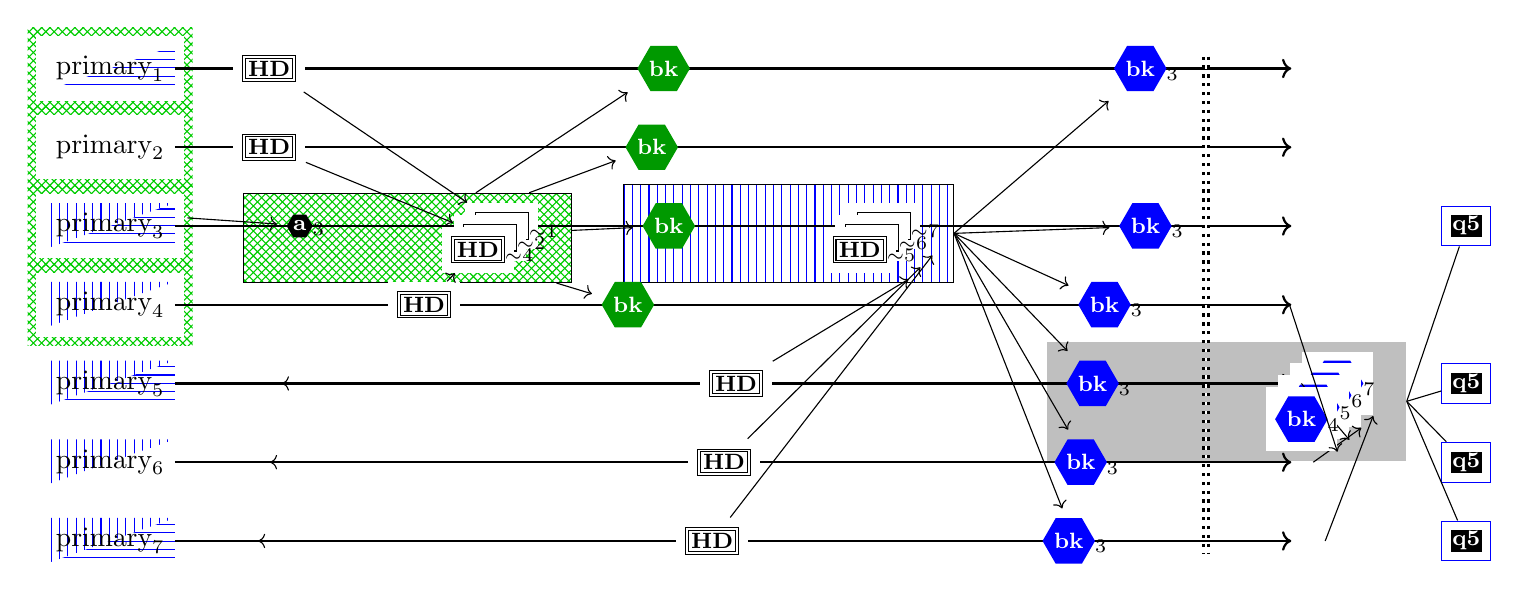
\begin{tikzpicture}[scale=1,thick]
      %%%%%%%%%%%%%%%%%%%%%%%%%%%%%%%%%%%%%%%%%%%%%%%%%%%%%%%%%%%%%%%%%%%%%%%%%%%%%%%%
      % The message passing diagram of the integrity protocol
      %%%%%%%%%%%%%%%%%%%%%%%%%%%%%%%%%%%%%%%%%%%%%%%%%%%%%%%%%%%%%%%%%%%%%%%%%%%
      \coordinate (primaryAnchor) at (0,0);
      \foreach \p in {1,...,7} {
        \node[below=\primaryDistance of primaryAnchor,anchor=east] (p\p)
        at (primaryAnchor) {\ensuremath{\text{primary}_\p}};
        \draw[->] (p\p) -- ++(15,0);
        \coordinate (primaryAnchor) at (p\p.east);
      }
      \begin{pgfonlayer}{background}
        \foreach \p in {1,...,4}{
          \node[pattern=crosshatch, pattern color=green!80!black,fit={(p\p)},inner sep=1.5ex] {};
          \node[fill=white, fit={(p\p)}] {};
        }
        \foreach \p in {1,3,5,7}{
          \fill[pattern=horizontal lines, pattern color=blue]
          (p\p.north east) -- (p\p.south west) -- (p\p.south east) -- cycle;
        }
        \foreach \p in {3,...,7}{
          \fill[pattern=vertical lines, pattern color=blue]
          (p\p.north east) -- (p\p.south west) -- (p\p.north west) -- cycle;
        }
      \end{pgfonlayer}

      \node[inner sep = 4ex] (theOrigin) at ([xshift=-3ex]p3.10) {};
      \foreach \p in {1,...,7} { % for each "other" validator
        \coordinate (ac\p') at ([xshift=17ex-\p ex]theOrigin|-p\p) ;
    }
    \node (ac3') at ([xshift=17ex-3 ex]theOrigin|-p3) {\ac\ensuremath{{}_3}};
    \draw[->] (theOrigin) -- ([xshift=4ex,yshift=4ex]ac3');
    \coordinate[right=14ex of ac3'] (sigAgg);
    \foreach \p in {1,2,4} { % for each "other" validator
      \node[fill=white] (av\p) at (sigAgg){\hd\makebox[0pt][l]{\ensuremath{{}_{\sim\p}}}};
      \coordinate (sigAgg) at ([xshift=-1ex,yshift=-1ex]sigAgg);
    }
    \foreach \p/\y in {1/2,2/1,4/-14} {
      \node[left=\y ex of ac\p',fill=white] (hd\p') {\hd};
      \draw[->] (hd\p') -- (av\p);
    }
    \begin{pgfonlayer}{background}
     
      \node[fit={(av4)([xshift=2ex]av1.north east)([xshift=-2ex]ac3'.west)},pattern=crosshatch,pattern color=green!80!black,draw] (bkGreen) {};
    \end{pgfonlayer}
    \foreach \p in {1,...,4} { % for each "green" validator
      \node[right=25 ex of ac\p'] (bkGreen\p') {\bk};
      \draw[->] (bkGreen) -- (bkGreen\p');
    }
    \foreach \p in {5,...,7} {
      \node[right=35 ex of ac\p',fill=white] (hd\p') {\hd};
      \draw[->] (hd\p') -- (ac\p');
    }
    \coordinate[right=15 ex of bkGreen3'] (sigAgg);
    \foreach \p in {7,...,5} { % for each "other" validator
      \node[fill=white] (av\p) at (sigAgg){\hd\makebox[0pt][l]{\ensuremath{{}_{\sim\p}}}};
      \draw[->] (hd\p') -- ([xshift=1ex,yshift=-.5ex]av\p.south east);
      \coordinate (sigAgg) at ([xshift=-1ex,yshift=-1ex]sigAgg);
    }
      \begin{pgfonlayer}{background}
       
        \node[fit={(bkGreen3')([xshift=2ex]av7.north east)(av5)},pattern=vertical lines,pattern color=blue,draw] (bkBlue) {};
      \end{pgfonlayer}
    \foreach \p in {7,...,3,1} { % for each validator in some "blue" quorum,
      \node[right=65 ex of ac\p'] (bkBlue\p') {\bk[blue]\ensuremath{{}_3}};
      \draw[->] (bkBlue.east) -- (bkBlue\p');
    }
    \coordinate (top) at (bkBlue3'.east|-p1);
    \coordinate (bottom) at (bkBlue3'.east|-p7);
    \draw[double,very thick,dotted] ([xshift=1ex,yshift=1ex]top) -- ([xshift=1ex,yshift=-1ex]bottom);
    \coordinate (sigAgg) at ([xshift=20ex]bkBlue5');
    \foreach \p in {7,...,4} { % for each "other" blue validator, not 3
      \node[fill=white] (bk\p) at (sigAgg){\bk[blue]\makebox[0pt][l]{\ensuremath{{}_\p}}};
      %\draw[->] (bk\p') -- ([xshift=1ex,yshift=-.5ex]av\p.south east);
      \coordinate (sigAgg) at ([xshift=-1ex,yshift=-1ex]sigAgg);
      \draw[->] (sigAgg|-p\p) -- (bk\p.south east);
    }   
    \begin{pgfonlayer}{background}
      \node[fit={(bkBlue5')([xshift=2ex]bk7.north east)(bk4.south west)},fill=lightgray] (BlueBlocks) {};
    \end{pgfonlayer}
    \foreach \p in {3,5,6,7} {% for some blue learners
      \node[draw=blue] (qs\p) at ([xshift=5ex]BlueBlocks.east|-p\p) {\qs[5]};
      \draw (BlueBlocks.east) -- (qs\p);
    }
  \end{tikzpicture}%
    \todo{for cooler patternage
      \url{https://tex.stackexchange.com/questions/597172/tikz-set-the-line-width-of-the-pattern}
    }
  }
  \caption[Integrity protocol]{%
    The integrity protocol
    (concluding each round that's was “opened” in the availability-protocol)%
  }
  %
  \label{fig:integrity-protocol}
\end{figure}

\subsection{Availability: the typical case for primaries}

\begin{description}
\item[Generating and broadcasting signed quorums]
  \xnote{primary \\⇒ primary}
  Once a validator has collected
  enough new  blocks (for a learner),
  it signs a learner-specific quorum of such blocks;
  the result is called a \emph{signed quorum}, 
  for short.
  All these blocks have to be from the same round. {\color{red} important ‼}

  Under certain conditions,
  in particular if there is exceptional delay for a specific learner,
  one can forgoe announcing a proper signed quorum
  and instead signs a \emph{dummy quorum} for a specific learner,
  \ie a signature over the ID of the learner in question and the current round number. 

\item[General header compilation]
  The biggest additional work and data
  concerns the compilation of headers.
  In the typical phase,
  a header carries two additional data items, namely
  \begin{itemize}
  \item
    the availability certificate of the previous header
    of the header's creator/initiator
  \item
    hashes of the signed (dummy) quorums sent by the same validator
  \end{itemize}

\item[General header checking]
  As signed quorums also serve as certificates of availability,
  checking a signed quorum amounts to checking the signed certificates.\endnote{%
    Somehow it seems overkill to have (hases of) signed quorums in the headers.   }
  In a similar way,
  the certificate of availability amounts to a checking of signatures.
\end{description}

\todo[inline]{describe in detail how

  the checking of the availability of the headers takes place}

\subsection{Summary}
The availability protocol in a non-genesis round
only differs in having
\begin{enumerate}
\item the additional requirement
that each block header also includes
the certificate of availability
for the previous header of the same validator and
\item
the sending and checking of signed quorums
(each of which implements the reference to
blocks from the previous round—in a learner-specific \Dag).
\end{enumerate}

As a consequence,
casting an availability vote / sending a commitment message
\todo{discuss terminnolgy}
becomes a recursive commitment
to storing all blocks until genesis
(or the last block that some of learners might still want availabl).

\section{Data structures}

\begin{figure}[htb]
  \centering
% \subfloat[\color{violet} \bf Missing]{
%   \begin{minipage}{.3\linewidth}
%       \begin{itemize}
%   \item Integrity Vote (cf. Availability Vote → Storing promise ?)
%   \item ~
%   \end{itemize}
%   \end{minipage}
% }

  \subfloat[Transaction received by worker~\(w\)]{
    \tx:
    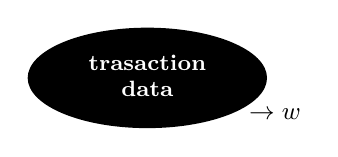
\begin{tikzpicture}[baseline={([yshift=-.5ex]b.center)}]
      \node[ellipse,fill=black] (b){
        \textcolor{white}{\bf\footnotesize\begin{tabular}[c]{c}
                                            trasaction\\
          data
        \end{tabular}}
    };
    \node[anchor=west] (w) at (b.south east) {\small\({}\to w\)};
    \end{tikzpicture}
  }
  \qquad
  \subfloat[Transaction copy (trivial erasure share)]{
    \es: \tx
    % \begin{tikzpicture}[baseline={([yshift=-.5ex]b.center)}]
    %   \phantom{
    %   \node[ellipse,fill=black] (b){
    %     \textcolor{white}{\bf\footnotesize\begin{tabular}[c]{c}
    %       blob\\
    %       of\\
    %       data
    %     \end{tabular}}
    %   };}
    % % https://texample.net/tikz/examples/torn-paper/
    % % ‼ make cute torn edges
    % \clip[fill] ([xshift=-1em]b.north east)
    % -- ([yshift=1em]b.south west)
    % -- ([xshift=1em]b.south west)
    % -- ([yshift=-1em]b.north east) -- cycle;
    % \node[ellipse,fill=black] (b){
    %     \textcolor{white}{\bf\footnotesize\begin{tabular}[c]{c}
    %       blob\\
    %       of\\
    %       data
    %     \end{tabular}}
    %   };
    % \end{tikzpicture}
}
  % \qquad
  % \subfloat[Worker \(y\) is commiting to the hash of~\(x\)]{
  %   \(y♯x\): \([\#(x)]_{\sim y}\)
  % }%‼

\subfloat[Batch hash of worker~\(w\)]{
  \#(\(\TXS\)):
  \#
    \(\left(\strut
          {\tx}:%\\%_{\to w}
          {\tx}:%\\%_{\to w}
          {\tx}:%\\%_{\to w}
          {\tx}:%\\%_{\to w}
          {\tx}:%\\%_{\to w}
          {\tx}%_{\to w}
          \right)\)
  }
  \subfloat[%
  Worker hash (broadcast by \(w\)),
  consisting of %
  the batch hash  \(\#\TXS\), %
  the batch number \(\bn\), %
  and the number of transactions \(\|\TXS\|\), %
  signed by~\(w\)]{
    \wh:
    \begin{tabular}[t]{@{}l@{}}
      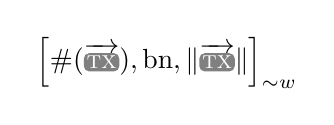
\begin{tikzpicture}[baseline={([yshift=-.5ex]wh.center)}]
        \node (wh){\(\left[ \#(\overrightarrow \tx), \bn,  \|\overrightarrow \tx\| \right]_{{\sim}w}\)};
      \end{tikzpicture}
      %\footnotesize
    % {\color{violet} + info for correctness checking} \\
    % (\eg number of \tx[s], or list of \#s)\\
    %   \emph{Tahoe – The Least-Authority Filesystem}
    \end{tabular}
  }

  \subfloat[Genesis Header]{
    \(\hd[]\):\(
\tikz[baseline={(x.base)}]{\node (x){
\(\left(p,\overrightarrow\wh\right)\)
};}\)
  }
\qquad
  \subfloat[Genesis certificate of availability]{
    \(\ac\):
    \(\Bigl[\hd[]\Bigr]_{\overrightarrow q}\)
  }

  \subfloat[Block]{
\bk:
    \begin{math}
      \left[\hd\right]_{\color{green!60!black}{\sim p_1 \dots \sim p_m} [ \color{green!60!black}\sim p_{m+1} \cdots \sim p_{k}]}
    \end{math}
  }
  \qquad
  \subfloat[Signed quorum]{
    \(\qs_p\):
    \begin{math}
      \begin{array}[c]{@{\rhd}l}
        [\bk_1 \cdots \bk_\ell]_{\sim p}
      \end{array}
    \end{math}
  }

  \subfloat[Header]{
    \(\hd\):\(
\tikz[baseline={(x.base)}]{\node (x){
\(\left(p,\overrightarrow\wh,\ac, \overrightarrow {\#(\qsₚ)}\right)\)
};}\)
  }


  \caption{Overview of data structures}
  \label{fig:data-structures}

\end{figure}

\FloatBarrier





\bibliographystyle{alpha}
\bibliography{HN.bib}

\appendix


\section{Message dependency management for actors}

\todo[inline]{%
  possibly move to the main part of the  paper %
  although it is technically not needed for the high(est)-level spec
}
Messages depending on other messages %
is a \emph{sine qua non} of consensus protocols. %
Typically,
sending a message according to some protocol %
is a reaction to having received one or several messages.\xspace%
\footnote{%
  Elapsing timers act very much like ``local messages'' %
  (cf.\ \statetright's \href%
  {docs.rs/stateright/latest/stateright/actor/trait.Actor.html}%
  {\texttt{on\_tiemeout}}%
  ). 
}
However, %
high-level protocol descriptions do not---and \emph{should} not---specify %
how a process can effectively become aware of the fact that %
it should send a specific message, %
let alone how it should keep track of all relevant received messages (efficiently). %
However, %
if we want to run the protocol, % 
we {have to} address these questions
by implementing what we call \emph{message dependency management}. %
We shall follow the actor based model, % 
which means that we have to map high-level protocol descriptions like
\emph{upon reception of header signatures from a weak quorum of validators} %
to a function that the processes calls for \emph{every} single received message %
and returns  a set of messages to be sent. 
%This amounts to specifying an actor based implementation of the protocol. %
We shall explain that %
it was indeed appropriate to disregard questions of message dependency management
``without loss of generality'' %
in our high-level description of \hnr. %

% When receiving a message, we have to first 
% the sender is aware of the fact that all messaged dependencies are met %
% and also can retrieve the received messages (from memory, storage, \etc). %
% Finally, %
% one has to have an efficient filter for irrelevant messages %
% (relative to the current observations of the agent). %

Let us look at some examples of message dependencies before %
we describe the complete message dependency manager.  %
\begin{ex}[Responses to header signature requests]
  Header signature requests (in the availability protocol)
  can only be answered (correctly) by a validator if
  it has received a confirmation from each of its workers.\footnote{
    Each confirmation states that
    a copy of the referenced transaction data has been stored.
  }
  This scenario is simple in that
  \begin{itemize}
  \item the primary knows exactly %
    which messages are expected from its workers; %
  \item each expected message's fingerprint is \emph{known in advance};
  \item there is only a single message to be synthesized and %
    it is known \emph{a priori}; % 
  \item progress towards meeting all dependencies is monotonic.
  \end{itemize}
  We can devise a relatively simple data structure:
  each expected message (fingerprint) is mapped to a pair of
  a shared counter and (a pointer to) the message to be signed.
  The counter is decremented of each one of the expected messages %
  and the message is synthesized. % 
\end{ex}

Now, if we look at availability certificates,
the situation becomes more tricky:
we are interested only in the first \(k\) messages out of \(n\);
moreover, 
the synthesized message depends on which messages turn out to be 
the first \(k\). 

\begin{ex}[Broadcasting certificates of availability (\textsc{i/ii})]
  Assuming that all validator sets of size~\(f+1\) (out of~\(3f+1\))
  form a weak quorum, we
  \begin{enumerate}
  \item count down a counter, starting from \(f+1\);
  \item synthesize the certificate of availability (and broadcast it)
    when the counter reaches \(0\);
  \item free the counter when it reaches~\(-2f\).
  \end{enumerate}
  There are optimizations to be made for the last point, 
  using a more efficient mechanism for identifying 
  messages that we can safely ignore. 
\end{ex}

In general, the situation becomes already a nightmare, %
if we consider fully general quorum systems. %
\todo[inline]{%
  probably kick this example out. 
}
\begin{ex}[Broadcasting certificates of availability (\textsc{ii/ii})]
  \todo{the below works only for systems in there is a single node in every
    quorum -- a veto node
    alternatively, one could put things ``upside down'',
    and let the leaves report on success -- 
    provided that every quorum has a node that does not belong to any other
    quorum (every neighborhood has a grumpy person)
  }\color{red}
  Assuming more general quorum systems,
  the idea of a simple counter does not work any more. %
  The brute force solution consists in using one counter for each quorum; %
  however, that would lead to an exponential blow-up. %
  Hence,
  we make use of the fact that
  each message falls into exactly one “region”\xspace%←that \xspace
  % allows do remove the footnote easily
  \footnote{%
    There is a one to one correspondence of regions and terms
    in the inclusion-exclusion formula,
    and \emph{vice versa}.
  }
  of the Venn diagram of all quorums. 
  Based on the
  \href%
  {https://en.wikipedia.org/wiki/Inclusion\%E2\%80\%93exclusion_principle}%
  {inclusion exclusion principle}, %
  we can organize the regions of the Venn diagram (of a set of subsets of a set)
  into a tree in which
  \begin{itemize}
  \item the root is the region of elements that belong to all sets
  \item the leaves are the regions of elements that belong to exactly one set
  \item there is a path from one region to another if the former is contained in
    every set that the latter is contained in
  \item in particular, the elements of a direct ancestor belong to exactly one additional set.
  \end{itemize}
  We set up a system of counters,
  one for each non-empty region,
  initialized to the size of the region.
  Each received signature contributes to exactly one counter,
  which is decremented upon message delivery. 
  Now,
  we have received enough signatures if, and only if, 
  all counters on a branch reach zero.
 \endnote{%
 \emph{On the inclusion exclusion principle.} %
   We can simplify this tree by repeating the following two operations,
   starting at the root:
   \begin{enumerate}
   \item coalesce all children of the same cardinality 
   \item coalesce parent and child if the child is the only child
   \end{enumerate}
   For a proper counter system, %
   we can disregard empty regions; %
   moreover,
   we can disregard empty regions. 
   Thus,
   we need at most one counter per learner. 
   Finally,
   counters organize into a tree in a natural way
   such that
   we have received enough signatures if, and only if, 
   all counters on a branch reach zero.
   \\\centerline{
     \colorbox{Apricot}{%
       \begin{tabular}[c]{p{20em}}
         Does the above algorithm (up to some corner case details of empty regions)
         yield a single node if we start with the set of all sub-sets?
       \end{tabular}
     }
   }
}
\end{ex}

We discern the following sub-tasks of message dependency management: %
filtering, trigger detection, message synthesis, (local) state update. %
\begin{description}
\item[Filtering] %
  How we can efficiently sort out irrelevant messages? %
\item[Trigger detection] %
  Is the received message a trigger for sending new messages?
\item[Message retrieval] %
  How can we retrieve exactly the relevant received messages?
\item[State update] %
  Update the local state for the above three processes to work. %
\end{description}
In fact, %
we update the state not in one single action, %
but divide it maintaining %
a ``database'' of messages on the one hand %
and accompanying triggering information on the other hand. %
Each trigger might result in a state update;
there may be a cascade of triggers
where, at least intuitively,
the triggered effect result in triggering new effects. %

\todo[inline,caption={}]{%
  revise this after going once through the protocol,
  filling descriptions of message dependencies
}

\begin{figure}[htb]
  \centering
    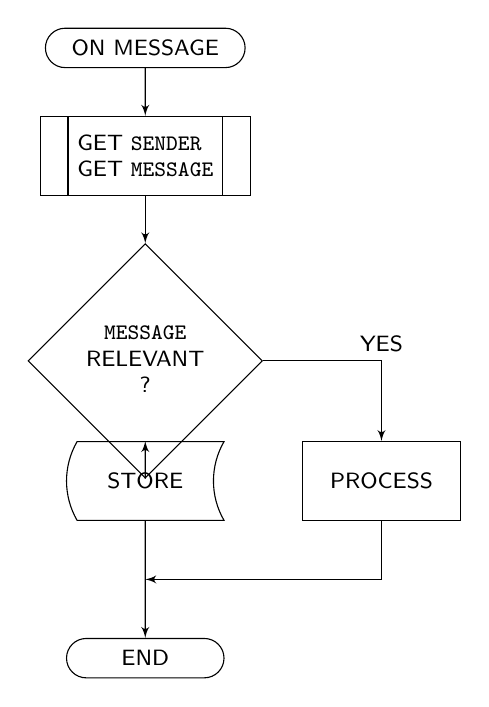
\begin{tikzpicture}[>=latex',font={\sf \footnotesize}]
      \def\smbwd{2cm}
      \node (terminal1) at (0,0) [draw, terminal,
      minimum width=\smbwd,
      minimum height=0.5cm] {ON MESSAGE};
      \node[below=4ex of terminal1] (predproc1) [%
      draw,%
      predproc,%
      align=left,%
      minimum width=\smbwd,%
      minimum height=1cm] {%
        GET \texttt{SENDER}\\%
        GET \texttt{MESSAGE}%
      }; 
      \node[below=4ex of predproc1] (decide1) [%
      draw, decision,
      minimum width=\smbwd,
      minimum height=1cm] {%
        \begin{tabular}[c]{@{}c@{}}%
          \texttt{MESSAGE}%
          \\%
          RELEVANT%
          \\?%
        \end{tabular}%
      };
      \node (storage1) at (0,-5.5) [draw, storage,
      minimum width=\smbwd,
      minimum height=1cm] {STORE};
      \node (process1) at (3,-5.5) [draw, process,
      minimum width=\smbwd,
      minimum height=1cm] {PROCESS};
      \coordinate (point1) at (0,-6.75);
      \node (terminal2) at (0,-7.75) [draw, terminal,
      minimum width=\smbwd,
      minimum height=0.5cm] {END};
      \draw[->] (terminal1) -- (predproc1);
      \draw[->] (predproc1) -- (decide1);
      \draw[->] (decide1) -| node[above]{YES} (process1);
      \draw[->] (decide1) -- (storage1);
      \draw[->] (process1) |- (point1);
      \draw[->] (storage1) -- (point1) -- (terminal2);
  \end{tikzpicture}
  \caption[Message dependency management]{Message dependency management:
    top-level flow chart}
  \label{fig:msg-dep-mng}
\end{figure}

In the accompanying %
\href%
{https://github.com/anoma/typhon/tree/hnarwhal-stateright}%
{prototype implementation}, %
these tasks are accomplished %
inside \statetright's \texttt{on\_msg}-functions. %


\begin{verbatim}
{
from [37] L. Zheng. Making distributed computation secure by construction. PhD thesis,
Cornell University, Ithaca, New York, USA, Jan. 2007.
}

4.4 Replication and message synthesis

Replicating code and data is an effective way to achieve
fault tolerance and ensure integrity and availability.
In DSR, both reactors and memory references may be replicated
on multiple hosts. Suppose reactor c is replicated on a set of hosts H.
Then other reactors interact with c as follows:
• Any message for c is sent to all the hosts in H.
• The replicas of c process incoming messages independently of each other. To
make this possible, all the program states of c have a local copy on every host in H.
In particular, every memory reference (location) accessed by c is also replicated
on H.
• If invoked with the same context identifier, the replicas of c are supposed to pro-
duce the same messages. Thus, the receiver host h of such a message µ may
receive the replicas of µ from different hosts in H. The redundancy is crucial
for achieving fault tolerance. Some hosts in H may be compromised, and these
bad hosts may send corrupted messages or simply not send anything. In general,
the replicas of µ received by h contain some correct ones, which are the same,
and some bad ones, which can be arbitrarily inconsistent. It is up to h to identify
the correct µ from those message replicas. This process is called message syn-
thesis, and the algorithm for identifying the correct message is called a message
synthesizer.
\end{verbatim}

\begin{verbatim}
message synthesizer ref(s)
  [37] L. Zheng. Making distributed computation secure by construction. PhD thesis,
  Cornell University, Ithaca, New York, USA, Jan. 2007.


  [39] L. Zheng and A. C. Myers. A language-based approach to secure quorum replication.
  In Proceedings of the Ninth Workshop on Programming Languages and Analysis for
  Security, PLAS’14, pages 27:27–27:39, New York, NY, USA, 2014. ACM. ISBN
  978-1-4503-2862-3. . URL http://doi.acm.org/10.1145/2637113.2637117.
\end{verbatim}

\section{Endnotes}
\printendnotes
\end{document}


%%% Local Variables:
%%% mode: latex
%%% TeX-master: t
%%% TeX-engine: luatex
%%% TeX-command-extra-options: "-shell-escape"
%%% End:





